\documentclass{article}

%headers and footers
\usepackage{fancyhdr}
\usepackage{array}
\pagestyle{fancyplain}

\usepackage{sidecap}
\usepackage{subfigure}
\usepackage{float}
\usepackage{longtable}
\usepackage{colortbl}
\usepackage{setspace}

\fancyhfoffset[LE, LO, RE, RO]{.1in}

\rhead{$671k4$}
\chead{}
\lhead{}

\lfoot{
\includegraphics[width=0.1\textwidth]{/home/zhangz/hts/scripts/bamchop.1.01/logo.jpg} {\bfseries Center for Biomedical Informatics at CHOP}}
\cfoot{}
\rfoot{\fancyplain{}{\thepage}}

\renewcommand{\footrulewidth}{0.4pt}

\addtolength{\voffset}{-54pt}
\addtolength{\hoffset}{-72pt}
\addtolength{\textwidth}{144pt}
\addtolength{\textheight}{108pt}


%hyperlink setup
\usepackage{hyperref}
\usepackage{xcolor}
\usepackage{underscore}
\usepackage{appendix}
\definecolor{dark-red}{rgb}{0.4,0.15,0.15}
\definecolor{dark-blue}{rgb}{0.15,0.15,0.4}
\definecolor{medium-blue}{rgb}{0,0,0.5}
\hypersetup{
  colorlinks, linkcolor={dark-red},
  citecolor={dark-blue}, urlcolor={medium-blue}
}

\setlength{\headheight}{10pt}
\setlength{\parindent}{0pt} 
\setlength{\parskip}{1ex}
\setlength{\tabcolsep}{5pt}
\setlength{\extrarowheight}{1.5pt}

\usepackage{Sweave}
\begin{document}
\begin{titlepage}
\title{ENCODE CD14+Monocyte Histone ChIP-seq: 671k4}
\author{Prepared by Zhe Zhang}
\maketitle
\tableofcontents
\end{titlepage}




\begin{center}
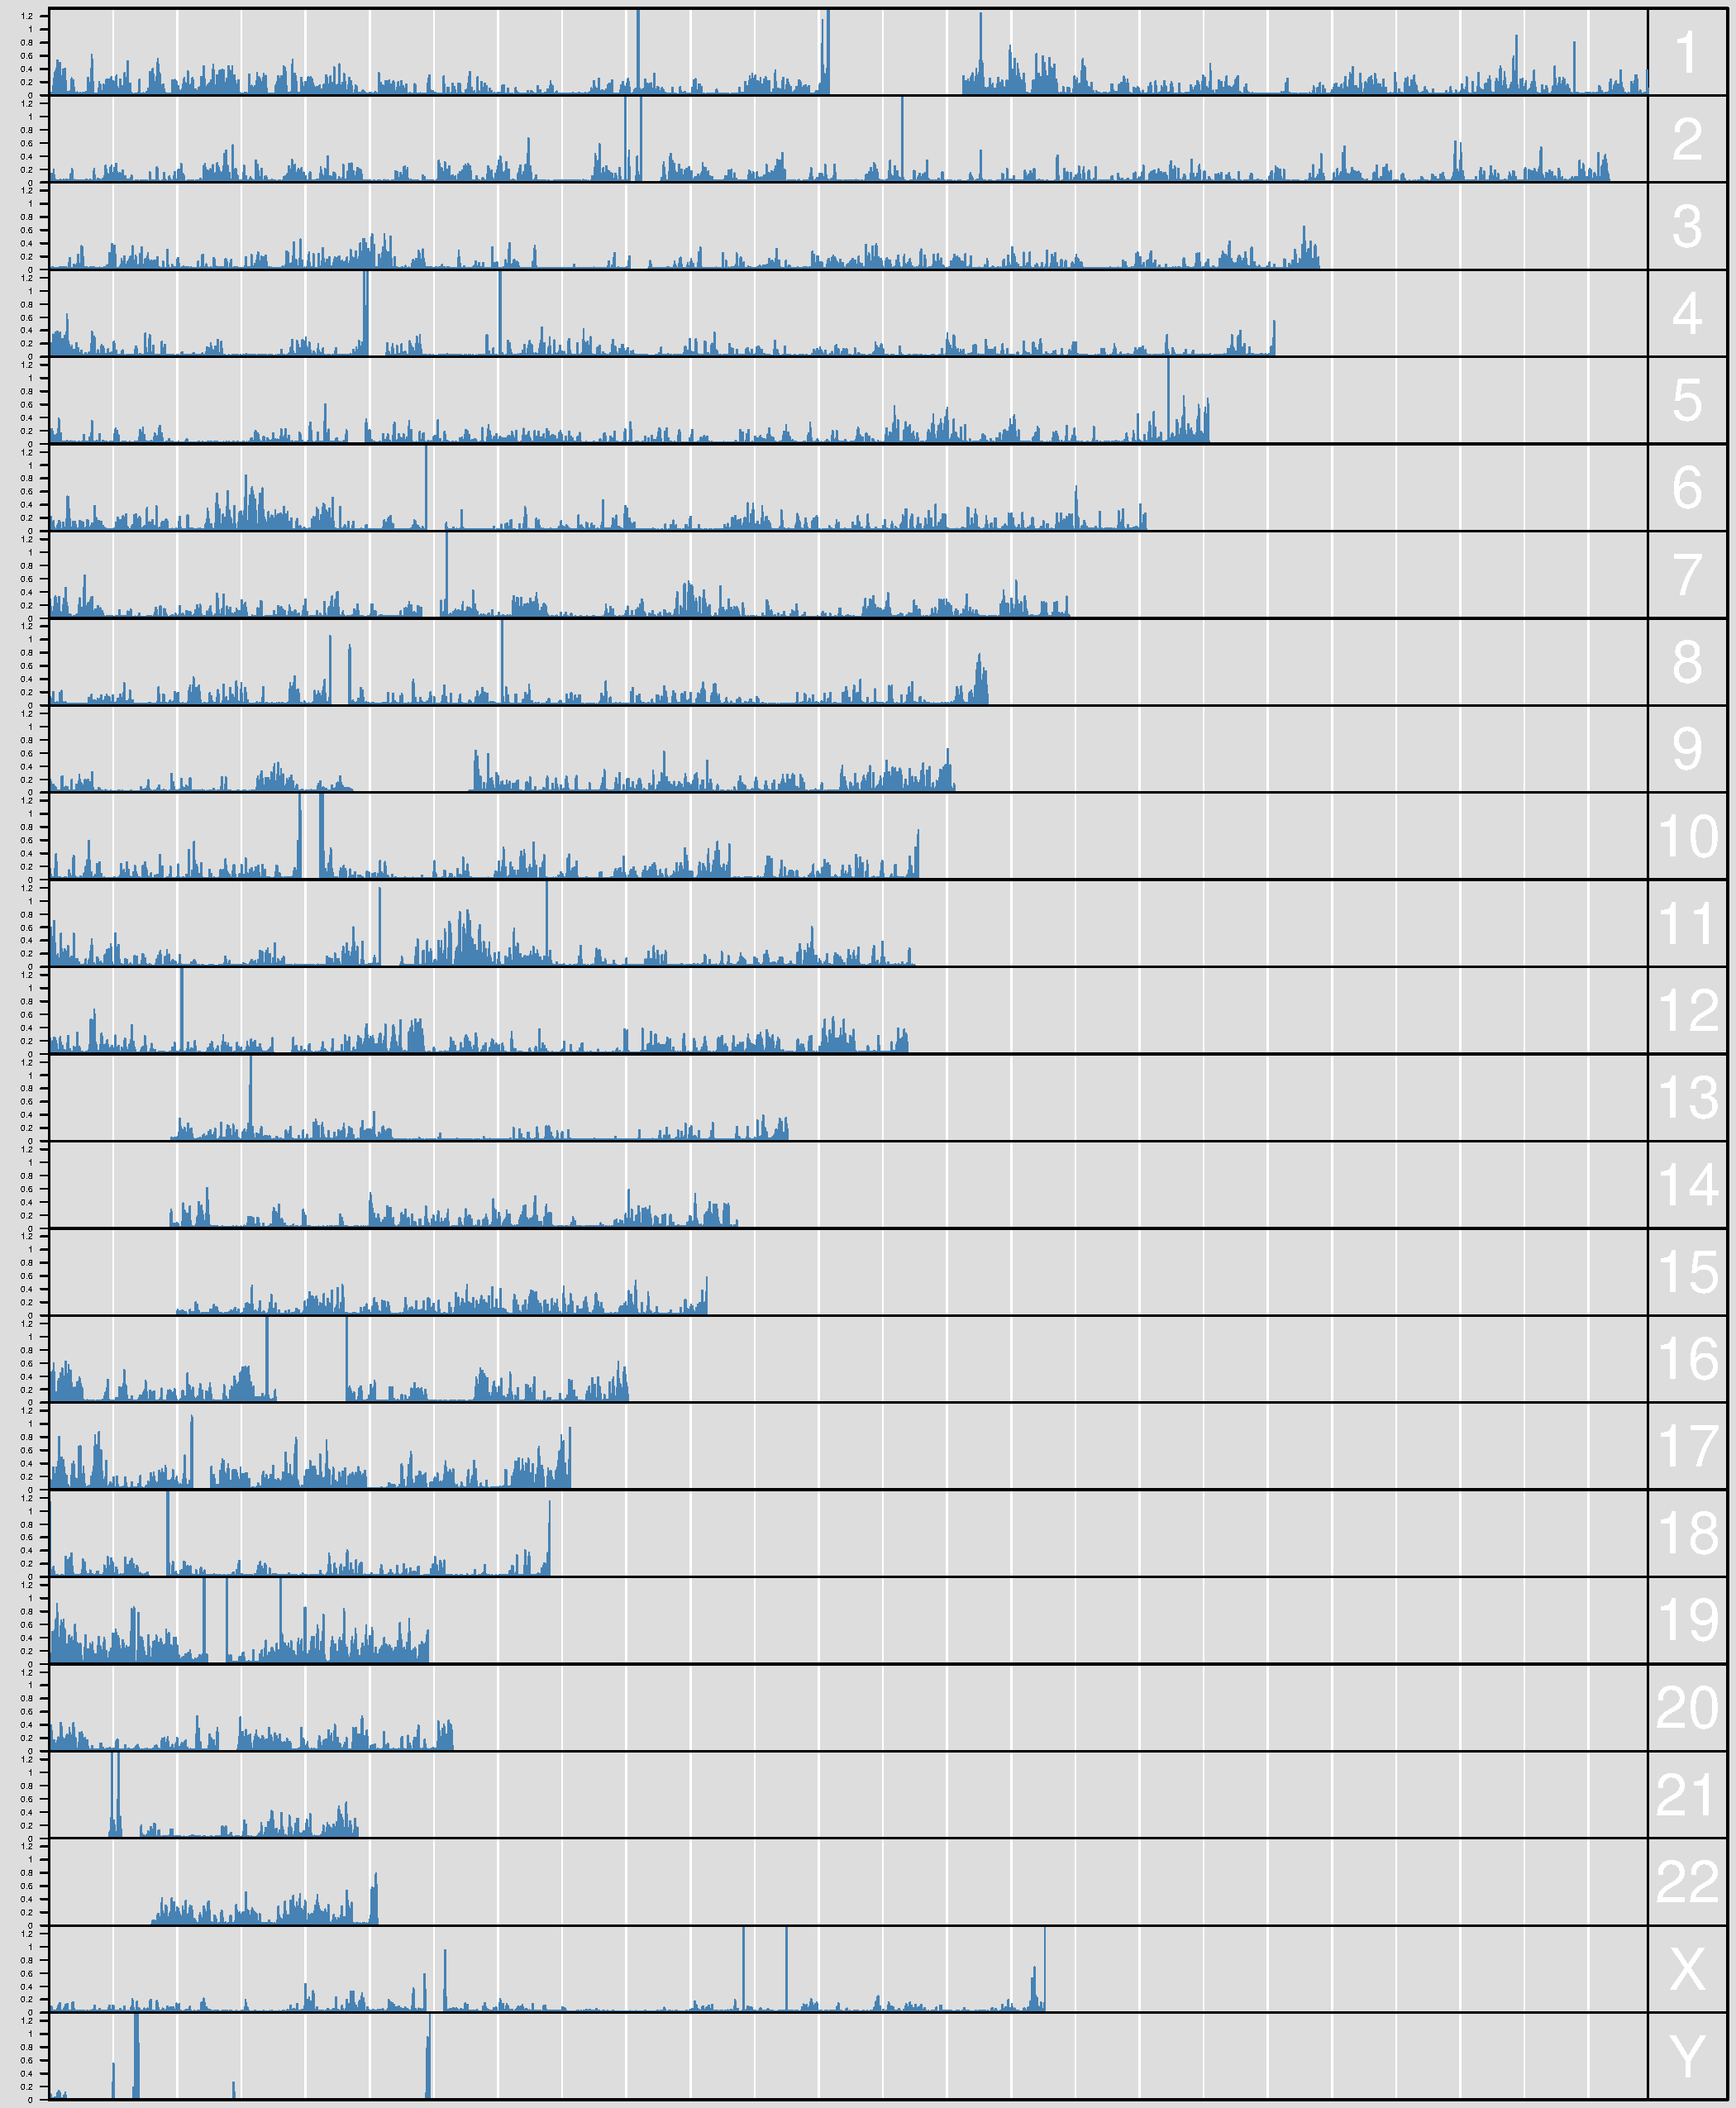
\includegraphics[width=7in, height=8.5in]{bamchop-landscape}
\end{center}
\pagebreak

\newpage
\section{Introduction}
\begin{description}
\item[\large{Project:}] 
\item[\large{Sample name:}] 671k4
\item[\large{Genome name:}] hg19
\end{description}

\subsection{BAM file}
\begin{description}
\item[\large{Size:}] 1.89 GB
\item[\large{Created:}] 2013-04-30 04:58:06
\item[\large{Modified:}] 2013-04-30 04:55:30
\item[\large{Location:}]  > home > zhangz > hts > projects > ks001 > 2013-04_BGI_ChIPseq > bams > novoalign_671k4_aligned.bam
\end{description}

\subsection{Summary statisitics}
\begin{SCtable}[1][h!]
% latex table generated in R 2.15.2 by xtable 1.7-0 package
% Tue Apr 30 10:15:20 2013
\begin{tabular}{|r|r|}
  \hline
  \rowcolor[gray]{0.9} \hline
Number of chromosomes & 24 \\ 
  Total reference size (bp) & 3,095,677,412 \\ 
   \rowcolor[gray]{0.9}Total effective size (bp) & 2,897,316,137 \\ 
  Total entries & 35,987,987 \\ 
   \rowcolor[gray]{0.9}Total mapped reads & 4,024,595 \\ 
  Total upmapped reads & 0 \\ 
   \rowcolor[gray]{0.9}Total mappings & 35,987,987 \\ 
  Total mapping locations & 3,636,721 \\ 
   \rowcolor[gray]{0.9}Base N\% & 0.003 \\ 
  (G+C)\% & 49.4 \\ 
   \rowcolor[gray]{0.9}Mapped to forward strand\% & 50.01 \\ 
  Duplicated mapping reads\% & 15.18 \\ 
   \rowcolor[gray]{0.9}Best sequencing quality & 41 \\ 
  Average sequencing quality & 38.62 \\ 
   \rowcolor[gray]{0.9}Maximum mapping length (bp) & 49 \\ 
  Minimum mapping length (bp) & 25 \\ 
   \rowcolor[gray]{0.9}Average mapping length (bp) & 48.75 \\ 
  Best mapping quality & 70 \\ 
   \rowcolor[gray]{0.9}Average mapping quality & 41.76 \\ 
  Highest sequencing depth & 9,207 \\ 
   \rowcolor[gray]{0.9}Average sequencing depth & 0.067 \\ 
  Mapped reads per kilobase & 1.39 \\ 
   \hline
\end{tabular}\caption{\textbf{Summary statistics}
\newline
\textbf{Effective size:} chromosome length without assembly gaps.
\newline
\textbf{Sequencing quality score:} assigned by the resequencing machine to indicate base calling confidence. 
\newline
\textbf{Mapping quality score:}  assigned by the alignment program to indicating mapping confidence.
\newline
\textbf{Mapping location:} strand-specific chromosomal location mapped to by the first base of one or more reads.
\newline
\textbf{Duplicated mapping:} the first base of multiple reads mapped to the same strand and chromosomal location.
}
\end{SCtable}

\pagebreak
\section{Read count and sequencing coverage}
This section summarizes the sequencing depth of reference chromosomes. Sequencing depth equals how many times a nucleotide base was sequenced.

\subsection{Depth categories}
\begin{SCtable}[1][!ht]
% latex table generated in R 2.15.2 by xtable 1.7-0 package
% Tue Apr 30 10:15:20 2013
\begin{tabular}{|r|r|r|}
  \hline
Depth & Count & Percentage \\ 
  \rowcolor[gray]{0.9} \hline
Depth=0 & 2,757,281,094 & 96.36 \\ 
  Depth$>$=1 & 104,051,512 &  3.64 \\ 
   \rowcolor[gray]{0.9}Depth$>$=5 & 7,965,969 &  0.28 \\ 
  Depth$>$=10 & 2,343,373 &  0.08 \\ 
   \rowcolor[gray]{0.9}Depth$>$=20 & 158,240 &  0.01 \\ 
  Depth$>$=30 & 59,483 &  0.00 \\ 
   \rowcolor[gray]{0.9}Depth$>$=50 & 28,317 &  0.00 \\ 
  Depth$>$=100 & 11,544 &  0.00 \\ 
   \rowcolor[gray]{0.9}Depth$>$=1000 & 1,505 &  0.00 \\ 
  Depth=9207 & 1 &  0.00 \\ 
   \hline
\end{tabular}\caption{\textbf{Depth by cutoffs.} Number and percentage of genomic locations (single bases) having the same or higher sequencing depth than given values.}
\end{SCtable}

\subsection{Depth by chromosome}
\begin{center}
% latex table generated in R 2.15.2 by xtable 1.7-0 package
% Tue Apr 30 10:15:20 2013
{\tiny
\begin{longtable}{|r|r|r|r|r|r|r|r|}
\caption{Sequencing depth by chromosome} \\ 
  \hline
Chromosome & Chromosome\_length & Effecitive\_size & Total\_reads & Unique\_mapping & Average\_depth & Maximum\_depth & Maximum\_location \\ 
  \hline
chr1 & 249,250,621 & 225,280,621 & 380,330 & 336,199 & 0.08 & 5,171 &  91,092,893 \\ 
   \rowcolor[gray]{0.9}chr2 & 243,199,373 & 238,207,373 & 316,633 & 276,057 & 0.06 & 4,560 & 128,285,576 \\ 
  chr3 & 198,022,430 & 194,797,140 & 224,128 & 211,253 & 0.06 &   280 & 193,460,439 \\ 
   \rowcolor[gray]{0.9}chr4 & 191,154,276 & 187,661,676 & 209,354 & 180,853 & 0.05 & 9,207 &  66,939,006 \\ 
  chr5 & 180,915,260 & 177,695,260 & 199,301 & 185,521 & 0.05 & 3,086 & 171,332,108 \\ 
   \rowcolor[gray]{0.9}chr6 & 171,115,067 & 167,395,067 & 216,505 & 202,220 & 0.06 & 1,140 & 130,184,090 \\ 
  chr7 & 159,138,663 & 155,353,663 & 201,745 & 189,134 & 0.06 &   246 &  58,669,049 \\ 
   \rowcolor[gray]{0.9}chr8 & 146,364,022 & 142,888,922 & 179,484 & 151,607 & 0.06 & 6,997 &  67,487,294 \\ 
  chr9 & 141,213,431 & 120,143,431 & 162,802 & 152,757 & 0.07 &   156 &  49,501,111 \\ 
   \rowcolor[gray]{0.9}chr10 & 135,534,747 & 131,314,747 & 200,153 & 173,943 & 0.07 &   947 &  39,020,268 \\ 
  chr11 & 135,006,516 & 131,129,516 & 193,613 & 177,708 & 0.07 & 2,341 &  73,980,570 \\ 
   \rowcolor[gray]{0.9}chr12 & 133,851,895 & 130,481,895 & 190,216 & 174,206 & 0.07 & 3,917 &  20,544,439 \\ 
  chr13 & 115,169,878 &  95,589,878 &  95,172 &  87,640 & 0.05 & 1,063 &  12,398,356 \\ 
   \rowcolor[gray]{0.9}chr14 & 107,349,540 &  88,289,540 & 120,560 & 111,765 & 0.07 & 1,688 &  71,341,410 \\ 
  chr15 & 102,531,392 &  81,694,769 & 118,062 & 111,238 & 0.07 &    40 &   8,264,635 \\ 
   \rowcolor[gray]{0.9}chr16 &  90,354,753 &  78,884,753 & 163,088 & 147,565 & 0.10 & 2,606 &  33,853,739 \\ 
  chr17 &  81,195,210 &  77,795,210 & 187,422 & 174,456 & 0.12 &   425 &  19,256,013 \\ 
   \rowcolor[gray]{0.9}chr18 &  78,077,248 &  74,657,248 &  80,723 &  72,850 & 0.05 &   642 &  74,656,465 \\ 
  chr19 &  59,128,983 &  55,808,983 & 205,189 & 178,995 & 0.18 & 5,476 &  23,974,122 \\ 
   \rowcolor[gray]{0.9}chr20 &  63,025,520 &  59,505,520 &  95,767 &  89,570 & 0.08 &   102 &  42,919,879 \\ 
  chr21 &  48,129,895 &  35,108,702 &  62,050 &  49,433 & 0.08 & 4,427 &     316,273 \\ 
   \rowcolor[gray]{0.9}chr22 &  51,304,566 &  34,894,566 &  74,133 &  69,418 & 0.10 &   127 &     661,655 \\ 
  chrX & 155,270,560 & 151,100,560 & 125,959 & 115,454 & 0.04 & 3,338 & 104,487,419 \\ 
   \rowcolor[gray]{0.9}chrY &  59,373,566 &  25,653,566 &  22,206 &  16,879 & 0.04 &   371 &  10,332,712 \\ 
   \hline
\hline
\end{longtable}
}\end{center}

\subsection{Depth by genomic feature}

\begin{center}
\begin{figure}[H]

\includegraphics[width=6.5in, height=4.5in, page=2]{bamchop-depth-feature}
\caption{\textbf{Average depth of genomic features.} Genomic features are regions annotated based on previous knowledge, such as the RefSeq gene track downloaded from UCSC genome browser. Many applications of high-throughput sequencing technologies, such as exome sequencing and RNA-seq, expect higher depth at exons.}
\end{figure}
\end{center}

\pagebreak

\section{Sequencing quality}
This section summarizes the sequencing quality scores assigned by the sequencer to single bases in each sequencing read and stored in the \textbf{<QUAL>} field of BAM files.
\vspace*{1\baselineskip}
\\{\textbf{Quality score summary:}}
\begin{Schunk}
\begin{Soutput}
   Min. 1st Qu.  Median    Mean 3rd Qu.    Max. 
   2.00   37.00   40.00   38.62   41.00   41.00 
\end{Soutput}
\end{Schunk}

\subsection{Quality score categories}
\begin{SCtable}[1][!ht]
% latex table generated in R 2.15.2 by xtable 1.7-0 package
% Tue Apr 30 10:15:20 2013
\begin{tabular}{|r|r|r|}
  \hline
Score & Count & Percentage \\ 
  \rowcolor[gray]{0.9} \hline
Score=0 &         0 &  0.00 \\ 
  Score$>$=5 & 7,075,182 & 99.83 \\ 
   \rowcolor[gray]{0.9}Score$>$=10 & 7,068,376 & 99.74 \\ 
  Score$>$=13 & 7,065,206 & 99.69 \\ 
   \rowcolor[gray]{0.9}Score$>$=20 & 7,047,871 & 99.45 \\ 
  Score$>$=30 & 6,956,591 & 98.16 \\ 
   \rowcolor[gray]{0.9}Score$>$=40 & 3,896,398 & 54.98 \\ 
  Score=41 & 3,023,200 & 42.66 \\ 
   \hline
\end{tabular}\caption{\textbf{Score categories.} The number and percentage of base calls having the quality socre equal to or higher than given values.)}
\end{SCtable}

\subsection{Overall score distribution}

\begin{center}
\begin{SCfigure}[1][!ht]
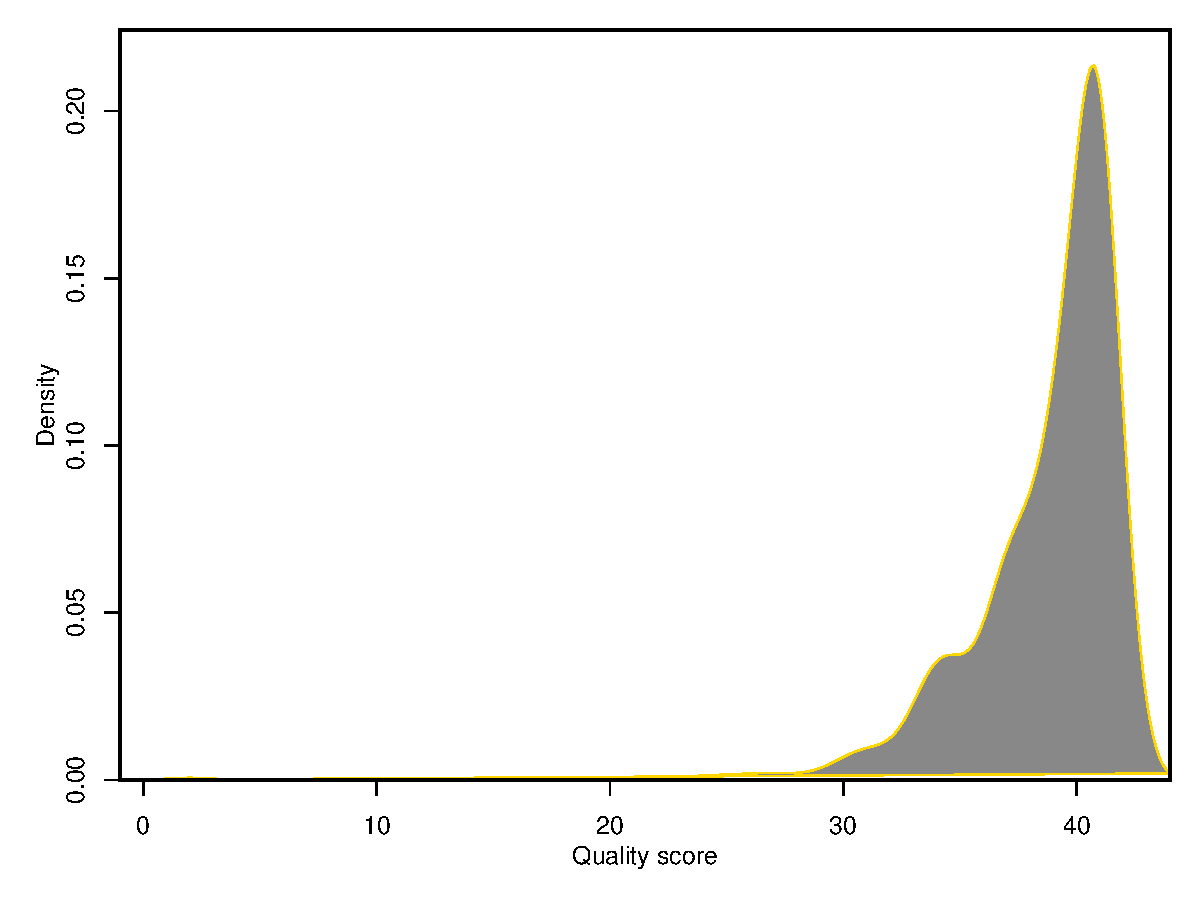
\includegraphics[width=4in, height=3in]{bamchop-qual-distribution}
\caption{\textbf{Score distribution.} This distribution is based on all bases of randomly selected sequencing reads, so position-specific sequencing quality is not considered (see below). The quality scores are calculated by subtracting 33 from the integers corresponding to the ASCII characters in \textbf{<QUAL>}. If the convention of Sanger sequencing was applied to generate the ASCII characters, they are equal to -10*Log10(p value), where p value is the likelihood of incorrect base call.}
\end{SCfigure}
\end{center}

\subsection{Position-specific score distribution}

\begin{center}
\begin{figure}[H]
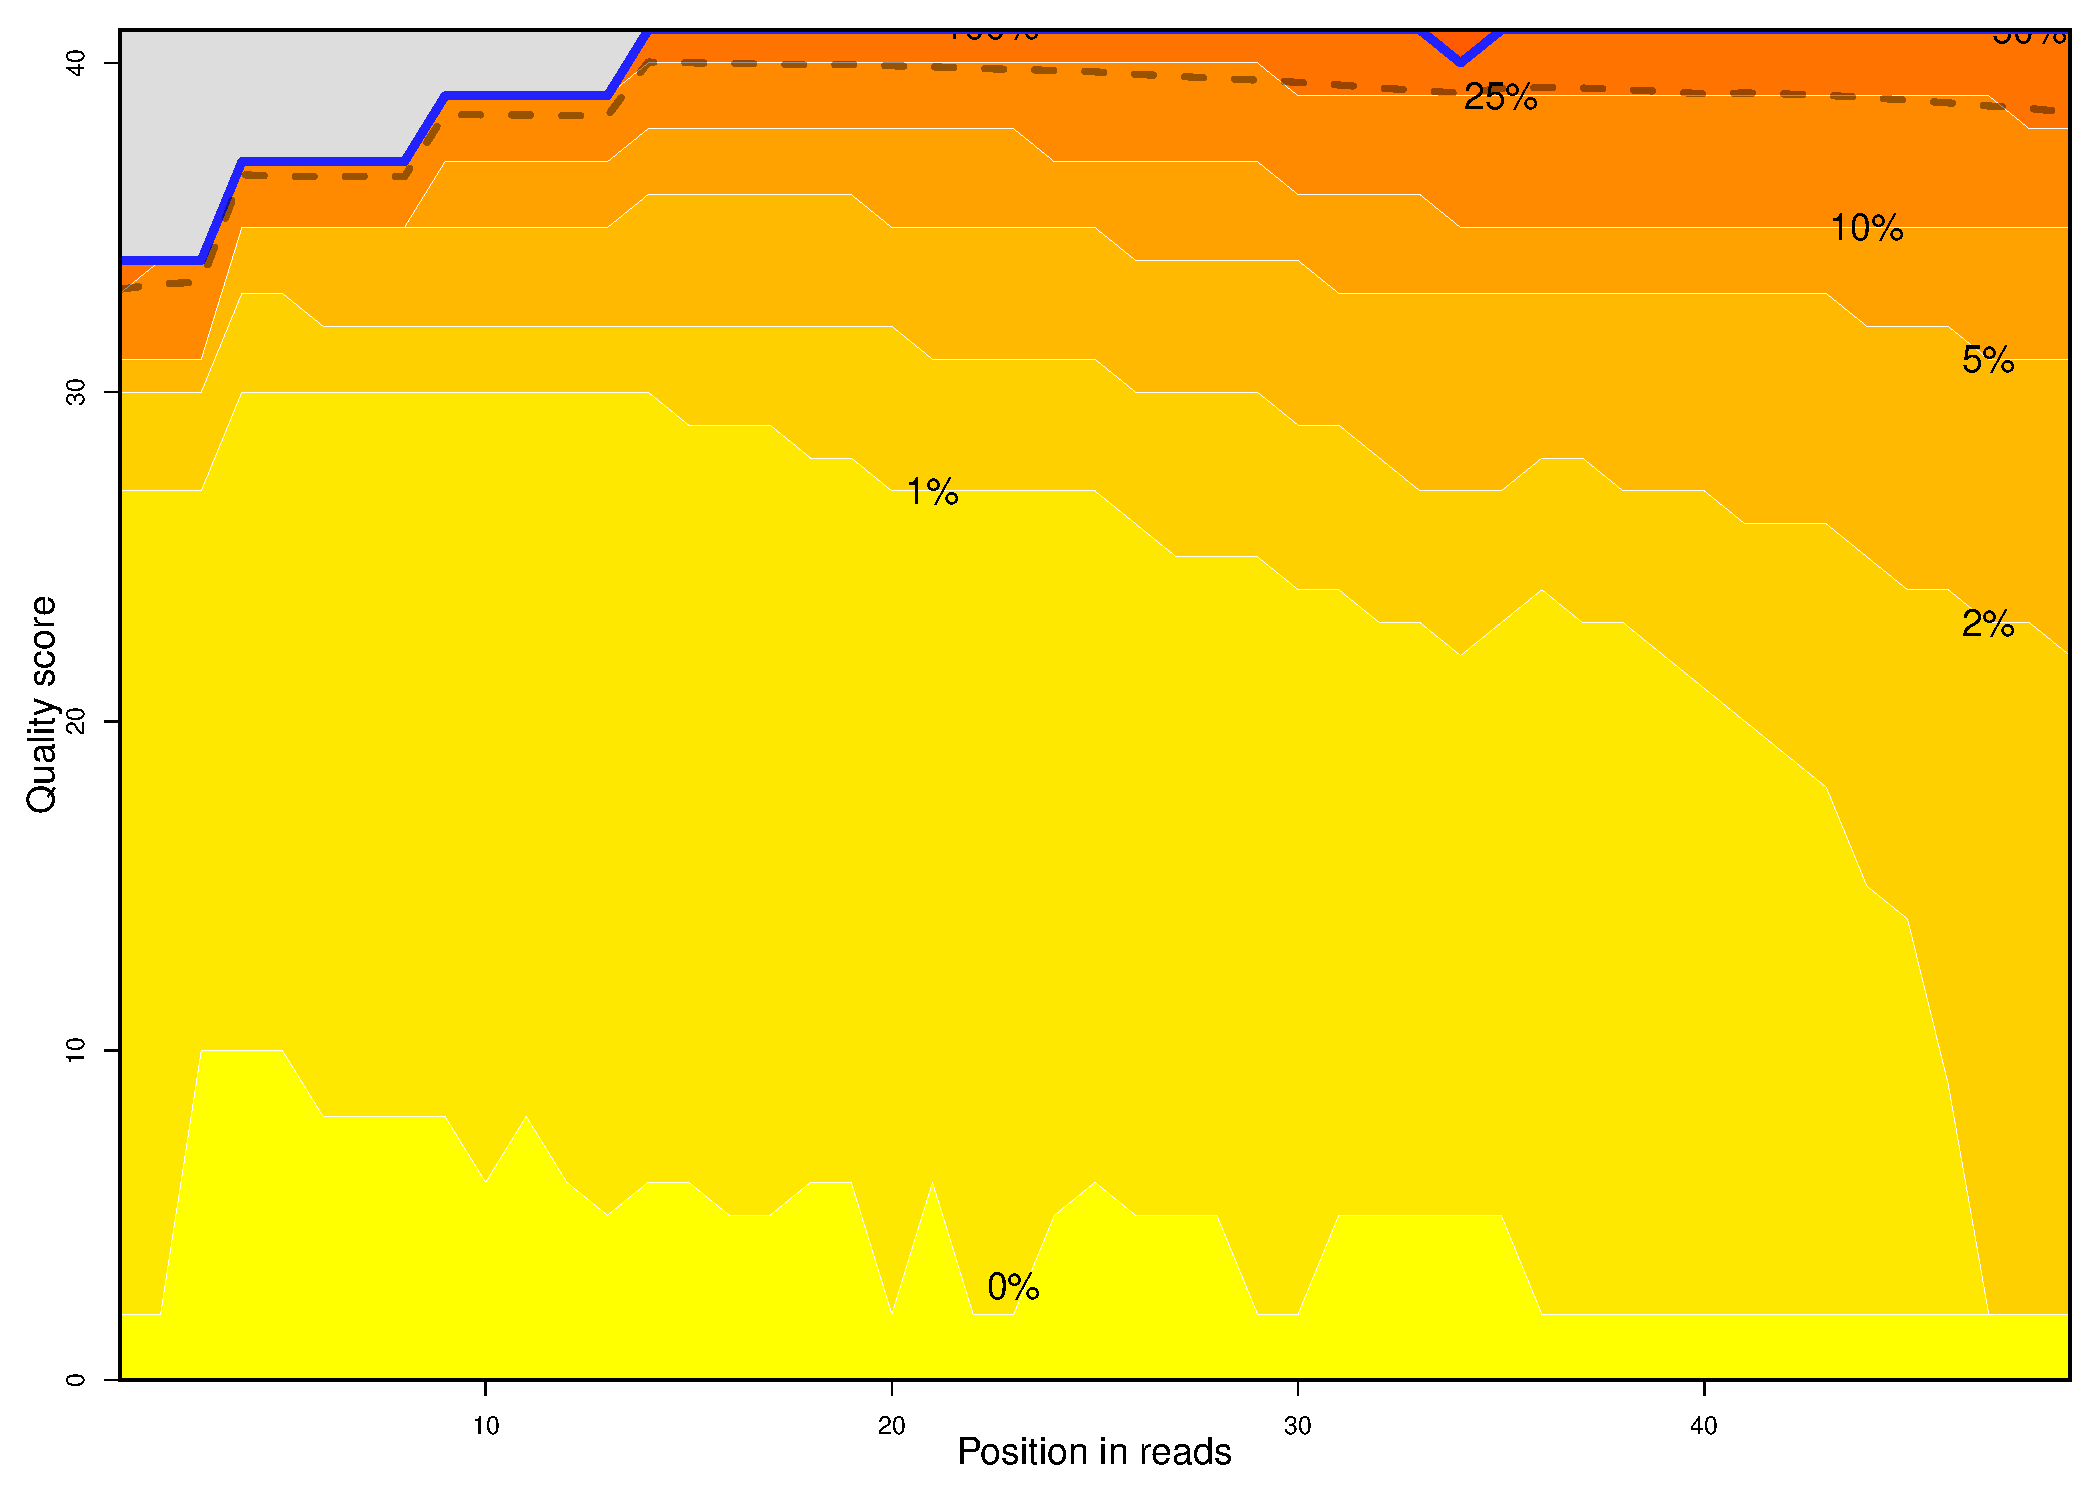
\includegraphics[width=7in, height=5in, page=1]{bamchop-qual-position}
\caption{\textbf{Position-specific sequencing scores.} This plot shows quality scores at different positions within reads. The dashed lines represents the means of quality scores at different positions; whereas the heat gradient corresponds to percentiles.}
\end{figure}
\end{center}


\pagebreak
\section{Mapping to reference}
This section summarizes the mapping of sequencing reads to reference chromosomes.
\subsection{Mapping length}
Mapping length corresponds to the \textbf{<QWIDTH>} field in BAM files, which is the number of bases in a read mapped to reference. Hard clipping reduces mapping length while soft clipping does not.
\vspace*{1\baselineskip}
\\{\textbf{Mapping length summary:}}
\begin{Schunk}
\begin{Soutput}
   Min. 1st Qu.  Median    Mean 3rd Qu.    Max. 
  25.00   49.00   49.00   48.75   49.00   49.00 
\end{Soutput}
\end{Schunk}


\begin{center}
\begin{figure}[H]
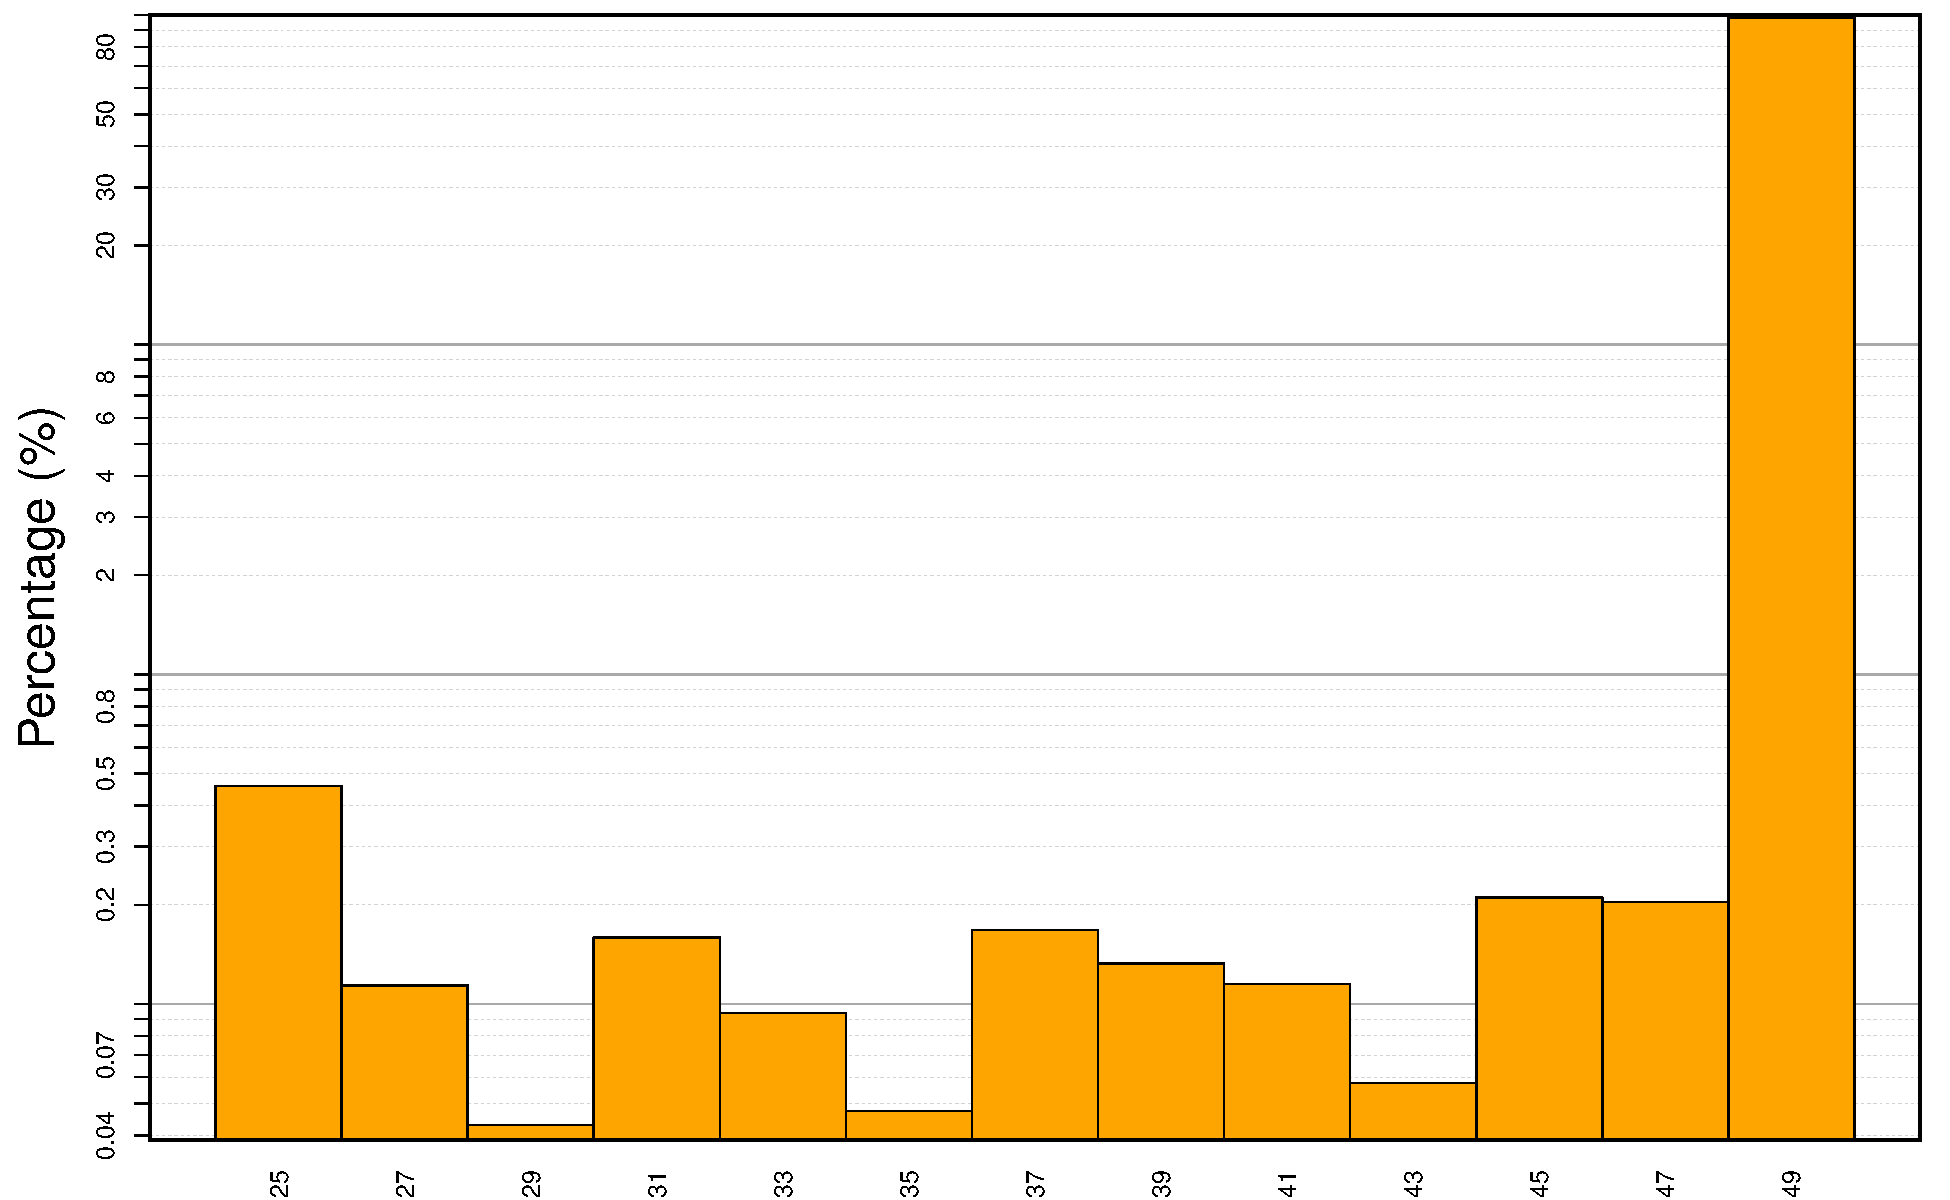
\includegraphics[width=6.5in, height=4in]{bamchop-mapping-length}
\caption{\textbf{Frequency of mapping lengths.} }
\end{figure}
\end{center}

\subsection{Mapping flag}
Mapping flag is stored in the \textbf{<FLAG>} field of BAM files. It uses a series of bitwise codes to represent different combinations of mapping results:
\begin{center}
% latex table generated in R 2.15.2 by xtable 1.7-0 package
% Tue Apr 30 10:15:20 2013
\begin{tabular}{ll}
  \hline
Bitwise & Description \\ 
  \hline
0X1 & template having multiple segments in sequencing \\ 
  0X2 & each segment properly aligned according to the aligner \\ 
  0X4 & segment unmapped \\ 
  0X8 & next segment in the template unmapped \\ 
  0X10 & SEQ being reverse complemented \\ 
  0X20 & SEQ of the next segment in the template being reversed \\ 
  0X40 & the first segment in the template \\ 
  0X80 & the last segment in the template \\ 
  0X100 & secondary alignment \\ 
  0X200 & not passing quality controls \\ 
  0X400 & PCR or optical duplicate \\ 
   \hline
\end{tabular}\end{center}

\subsubsection{Mapping flag categories}
\begin{SCtable}[1][h!]
% latex table generated in R 2.15.2 by xtable 1.7-0 package
% Tue Apr 30 10:15:20 2013
\begin{tabular}{|r|r|r|}
  \hline
Code & Count & Percentage \\ 
  \rowcolor[gray]{0.9} \hline
0X1 &          0 &  0.00 \\ 
  0X2 &          0 &  0.00 \\ 
   \rowcolor[gray]{0.9}0X4 &          0 &  0.00 \\ 
  0X8 &          0 &  0.00 \\ 
   \rowcolor[gray]{0.9}0X10 & 17,989,389 & 49.99 \\ 
  0X20 &          0 &  0.00 \\ 
   \rowcolor[gray]{0.9}0X40 &          0 &  0.00 \\ 
  0X80 &          0 &  0.00 \\ 
   \rowcolor[gray]{0.9}0X100 & 31,963,392 & 88.82 \\ 
  0X200 &          0 &  0.00 \\ 
   \rowcolor[gray]{0.9}0X400 &          0 &  0.00 \\ 
   \hline
\end{tabular}\caption{\textbf{Mapping flag categories.} The total number and percentage of reads flagged by each category.}
\end{SCtable}

\subsubsection{Flag value breakdown}
\begin{center}
% latex table generated in R 2.15.2 by xtable 1.7-0 package
% Tue Apr 30 10:15:20 2013
{\tiny
\begin{longtable}{|r|r|r|r|r|r|r|r|r|r|r|r|r|r|}
\caption{The breakdown of values into flag categories.} \\ 
  \hline
Value & Count & Percentage & 0X1 & 0X2 & 0X4 & 0X8 & 0X10 & 0X20 & 0X40 & 0X80 & 0X100 & 0X200 & 0X400 \\ 
  \hline
0 &  2,010,196 &  5.59 & - & - & - & - & - & - & - & - & - & - & - \\ 
   \rowcolor[gray]{0.9}16 &  2,014,399 &  5.60 & - & - & - & - & X & - & - & - & - & - & - \\ 
  256 & 15,988,402 & 44.43 & - & - & - & - & - & - & - & - & X & - & - \\ 
   \rowcolor[gray]{0.9}272 & 15,974,990 & 44.39 & - & - & - & - & X & - & - & - & X & - & - \\ 
   \hline
\hline
\end{longtable}
}\end{center}

\subsection{Mapping score}
Mapping scores are assigned by the alignment program to indicate the likelihood of false alignment and stored in the \textbf{<MAPQ>} field of BAM files. Higher score usually means longer alignment, less mismatch, and/or higher uniqueness. 
\vspace*{1\baselineskip}
\\{\textbf{Mapping score summary:}}
\begin{Schunk}
\begin{Soutput}
   Min. 1st Qu.  Median    Mean 3rd Qu.    Max. 
   0.00    0.00   70.00   41.76   70.00   70.00 
\end{Soutput}
\end{Schunk}

\subsubsection{Mapping score categories}
\vspace*{1\baselineskip}
\begin{SCtable}[1][!ht]
% latex table generated in R 2.15.2 by xtable 1.7-0 package
% Tue Apr 30 10:15:20 2013
\begin{tabular}{|r|r|r|}
  \hline
Score & Count & Percentage \\ 
  \rowcolor[gray]{0.9} \hline
mapq=0 & 45,533 & 31.43 \\ 
  mapq$>$=1 & 99,325 & 68.57 \\ 
   \rowcolor[gray]{0.9}mapq$>$=2 & 95,969 & 66.25 \\ 
  mapq$>$=3 & 94,514 & 65.25 \\ 
   \rowcolor[gray]{0.9}mapq$>$=4 & 91,808 & 63.38 \\ 
  mapq$>$=5 & 91,759 & 63.34 \\ 
   \rowcolor[gray]{0.9}mapq$>$=10 & 91,489 & 63.16 \\ 
  mapq$>$=20 & 89,654 & 61.89 \\ 
   \rowcolor[gray]{0.9}mapq$>$=30 & 85,866 & 59.28 \\ 
  mapq$>$=40 & 85,053 & 58.71 \\ 
   \rowcolor[gray]{0.9}mapq=70 & 80,900 & 55.85 \\ 
   \hline
\end{tabular}\caption{\textbf{Mapping score categories.} The total number and percentage of reads having mapping scores equal to or higher than given values.}
\end{SCtable}

\subsubsection{Overall score distribution}

\begin{center}
\begin{figure}[H]
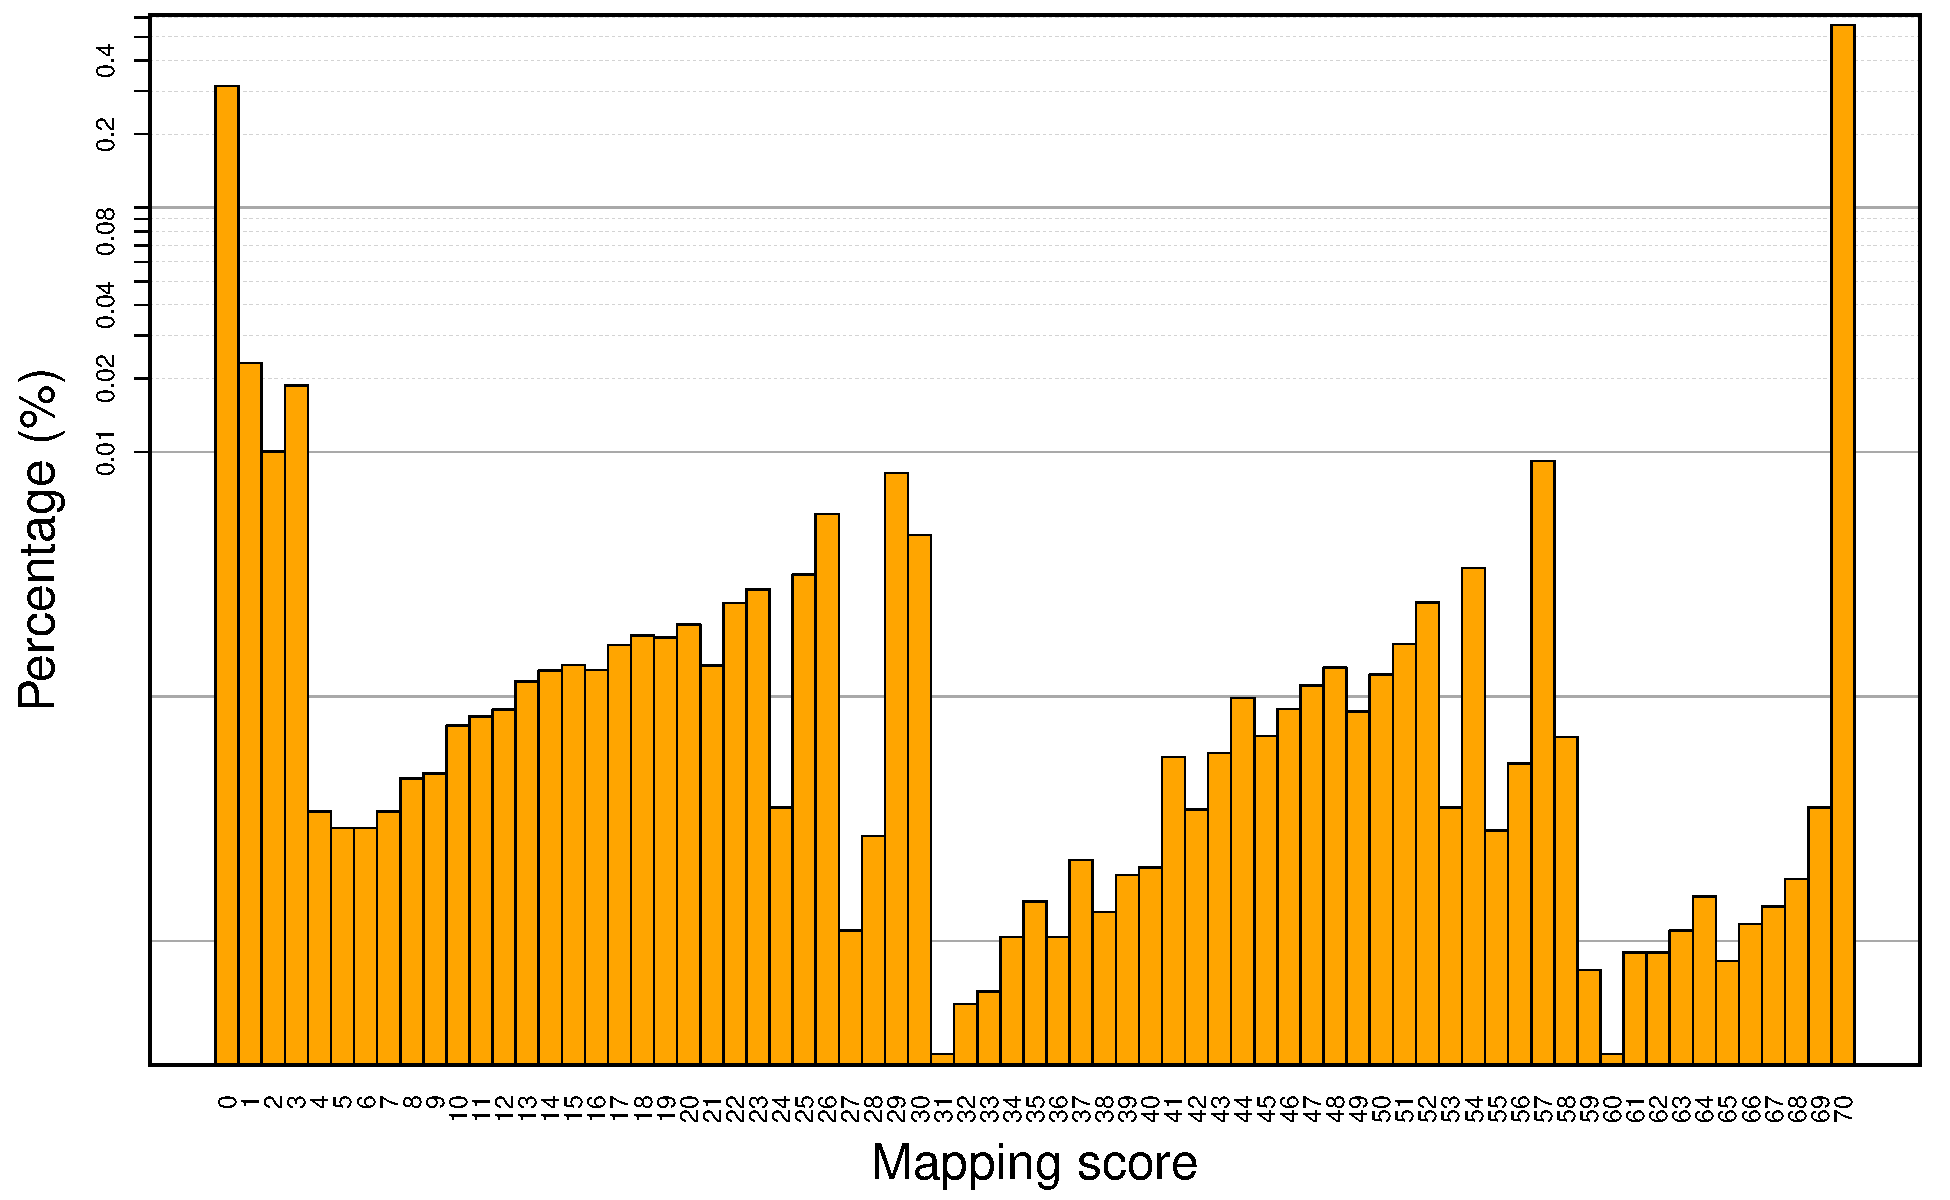
\includegraphics[width=6.5in, height=4in]{bamchop-mapq-distribution}
\caption{\textbf{Mapping score distribution. } By definition, mapping quality equals to -10*Log10(p value), where p value is the likelihood of incorrect mapping; however, its calculation depends on individual programs.}
\end{figure}
\end{center}

\subsection{Mismatch (CIGAR)}
SAM uses the \textbf{<CIGAR>} field to compactly represent alignments. CIGAR characters are used in concert with lengths to describe various types of matching, mismatching, clipping, padding and splicing events within an alignment.
\subsubsection{Mismatch categories}
\begin{center}
% latex table generated in R 2.15.2 by xtable 1.7-0 package
% Tue Apr 30 10:15:20 2013
\begin{tabular}{ll}
  \hline
Bitwise & Description \\ 
  \hline
M & alignment match (can be a sequence match or mismatch) \\ 
  I & insertion to the reference \\ 
  D & deletion from the reference \\ 
  N & skipped region from the reference \\ 
  S & soft clipping (clipped sequences present in SEQ) \\ 
  H & hard clipping (clipped sequences NOT present in SEQ) \\ 
  P & padding (silent deletion from padded reference) \\ 
  = & sequence match \\ 
  X & sequence mismatch \\ 
   \hline
\end{tabular}\end{center}

\begin{SCtable}[1][h!]
% latex table generated in R 2.15.2 by xtable 1.7-0 package
% Tue Apr 30 10:15:20 2013
\begin{tabular}{|r|r|r|}
  \hline
Category & Count & Percentage \\ 
  \rowcolor[gray]{0.9} \hline
M & 4,024,595 & 100.00 \\ 
  I &    26,881 &   0.67 \\ 
   \rowcolor[gray]{0.9}D &    13,704 &   0.34 \\ 
  S &   284,454 &   7.07 \\ 
   \rowcolor[gray]{0.9}H &    72,565 &   1.80 \\ 
   \hline
\end{tabular}\caption{\textbf{Mismatch categories} The total number and percentage of reads having specific types of mismatches.}
\end{SCtable}

\subsubsection{Gapped alignment}
\textbf{Not reads having gapped alignment.}

\begin{center}
\begin{SCfigure}[1][h!]
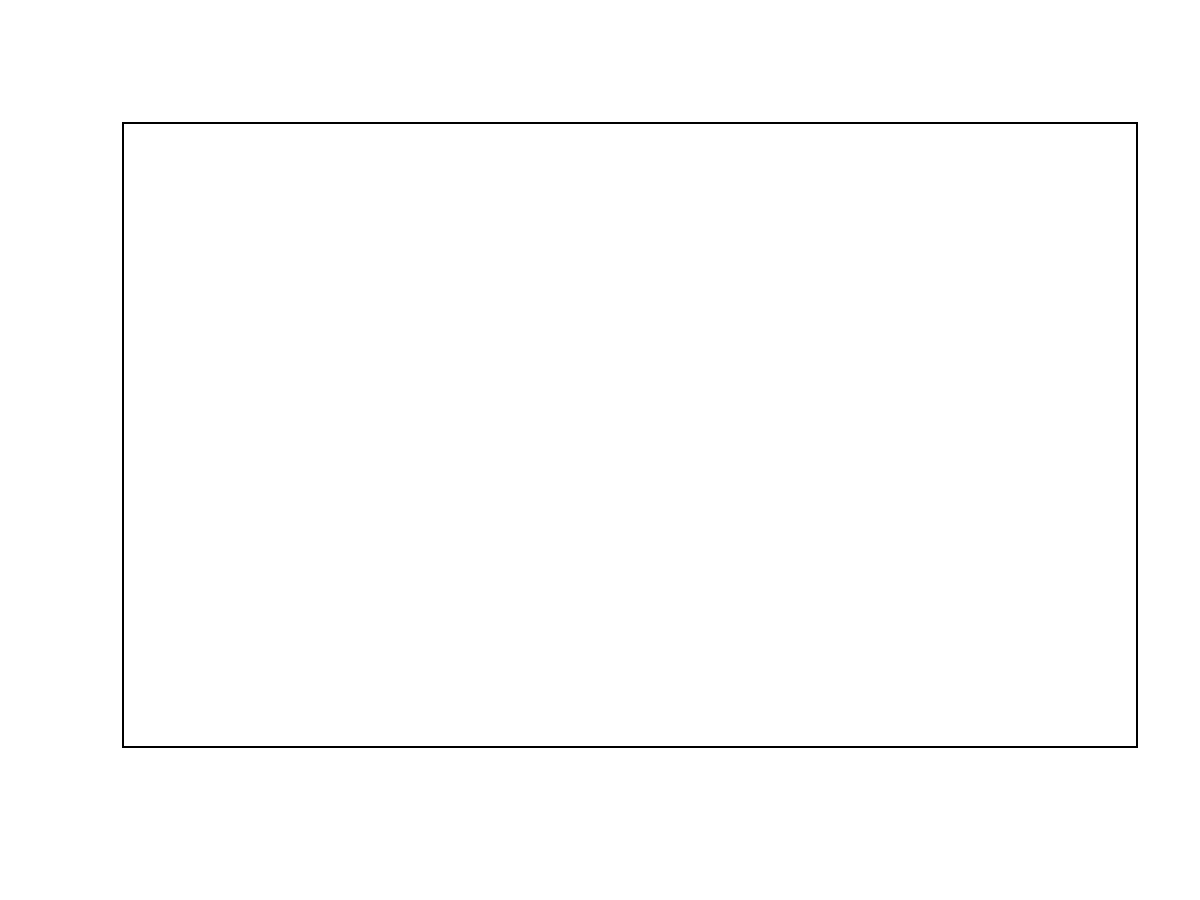
\includegraphics[width=4in, height=3in]{bamchop-gap-size}
\caption{\textbf{Distribution of gap size.} If the alignment program tried to align sub-sequence of the same read to remote locations, \textbf{<CIGAR>} will provide the size of gapped regions}
\end{SCfigure}
\end{center}


\subsection{Duplicated mapping}
Duplicated mapping refers to multiple reads having their first base mapped to the same strand and location. Duplication level is the number of reads sharing the same duplicated mapping. It is an indicator of the effect of PCR artifact, but also depends on local and overall sequencing depth.

\subsubsection{Duplication level categories}
\textbf{The average number of duplicated reads at each mapping location is 1.107.}
\begin{SCtable}[1][h!]
% latex table generated in R 2.15.2 by xtable 1.7-0 package
% Tue Apr 30 10:15:20 2013
\begin{tabular}{|r|r|r|r|}
  \hline
Level & Location\_count & Read\_count & Percentage \\ 
  \rowcolor[gray]{0.9} \hline
1 & 3,413,810 & 3,413,810 & 84.82 \\ 
  2 & 194,981 & 389,962 &  9.69 \\ 
   \rowcolor[gray]{0.9}3 & 17,495 & 52,485 &  1.30 \\ 
  4 & 3,620 & 14,480 &  0.36 \\ 
   \rowcolor[gray]{0.9}5 & 1,611 & 8,055 &  0.20 \\ 
  6 & 981 & 5,886 &  0.15 \\ 
   \rowcolor[gray]{0.9}7 & 575 & 4,025 &  0.10 \\ 
  8 & 455 & 3,640 &  0.09 \\ 
   \rowcolor[gray]{0.9}9 & 315 & 2,835 &  0.07 \\ 
  10 & 243 & 2,430 &  0.06 \\ 
   \rowcolor[gray]{0.9}$>$10 & 2,635 & 126,987 &  3.16 \\ 
   \hline
\end{tabular}\caption{\textbf{Duplication level categories.} Numbers of mapping locations and reads having the duplication levels of the given values.}
\end{SCtable}

\subsubsection{Overall duplication distribution}

\begin{center}
\begin{figure}[H]
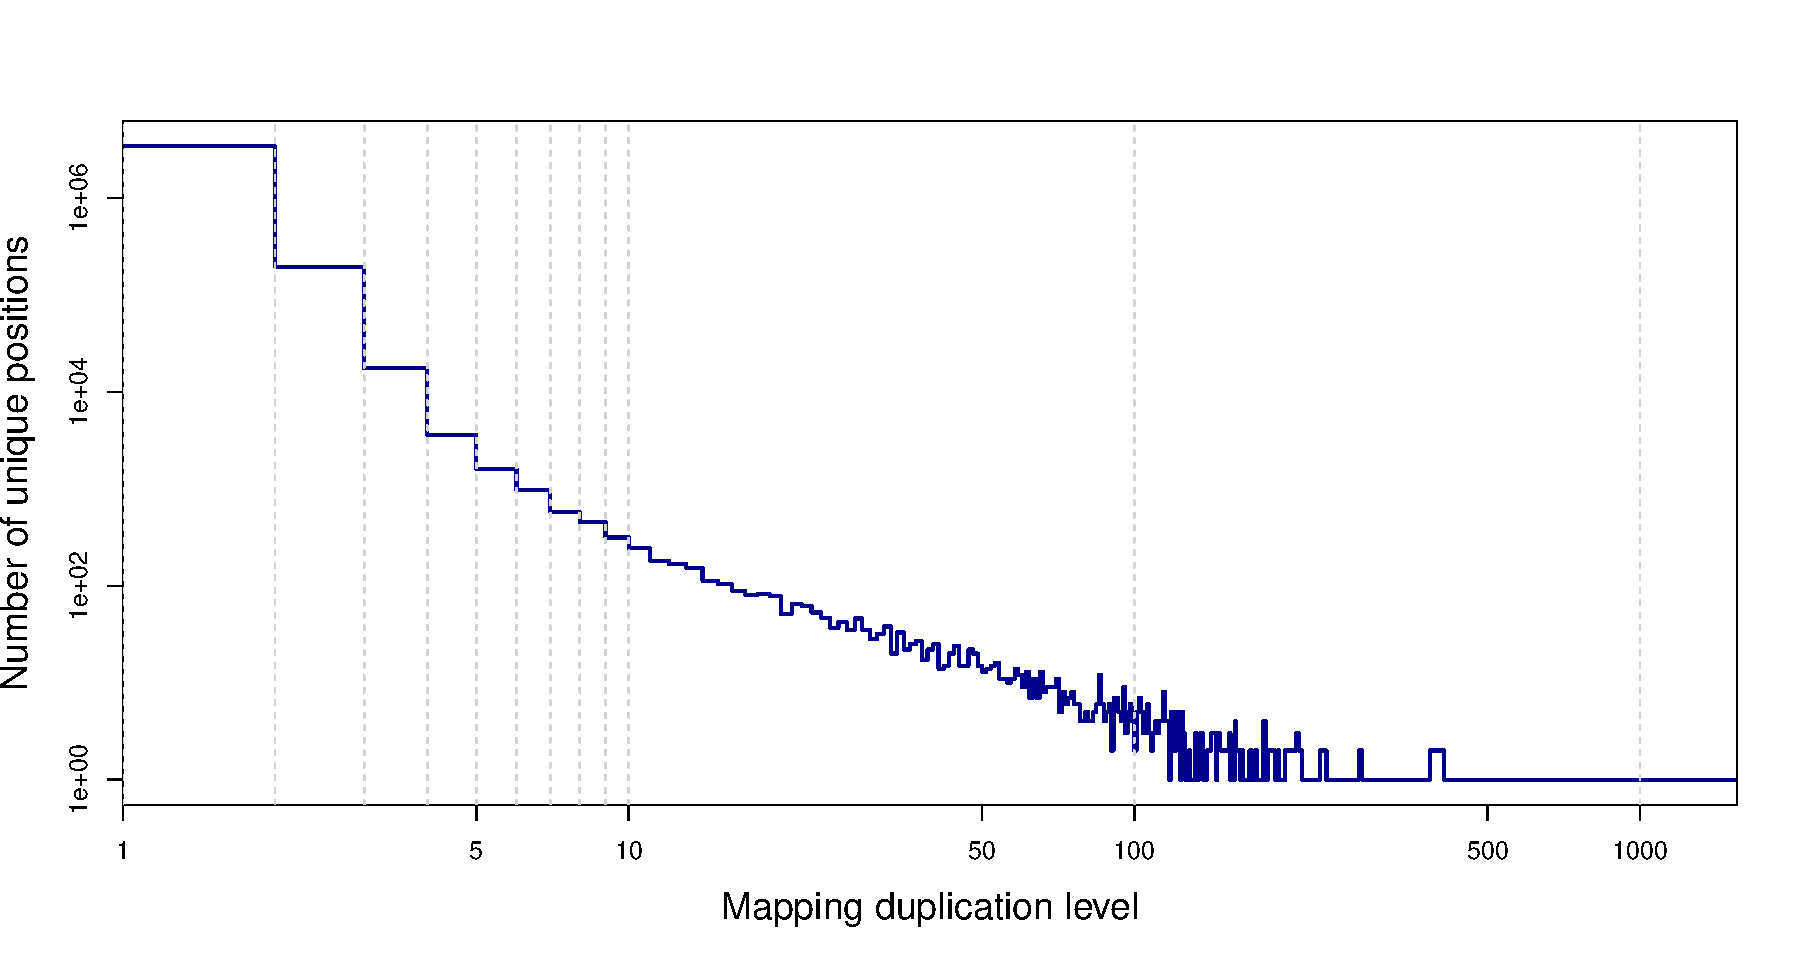
\includegraphics[width=6in, height=3.2in]{bamchop-dup-distribution}
\caption{textbf{Distribution of duplication levels}. The x-axis indicates the number of reads sharing the same mapping location of their 5'-end and the y-axis is the total occurance of each level. Only reads mapped to the forward strand and the first 10 million reads of each chromosome was used to reduce computation.}
\end{figure}
\end{center}

\subsection{Paired reads}
\textbf{No information about paired-end reads is available in this BAM file.}

\subsubsection{Read count summary}
\textbf{Not applicable.}
\begin{SCtable}[1][h!]
% latex table generated in R 2.15.2 by xtable 1.7-0 package
% Tue Apr 30 10:15:20 2013
\begin{tabular}{|r|r|r|}
  \hline
Category & Count & Percent \\ 
  \rowcolor[gray]{0.9} \hline
Total paired-end reads & 0.00 & 0.00 \\ 
   \hline
\end{tabular}\caption{\textbf{Paired-end reads.} Read counts in this table are based on the "flag" field in BAM file. Properly mapping paired-end reads are reads mapped to the opposite strand of the same chromosome. }
\end{SCtable}

\subsubsection{Insertion size of paired reads}
\textbf{Not applicable.}


\begin{center}
\begin{SCfigure}[1][h!]
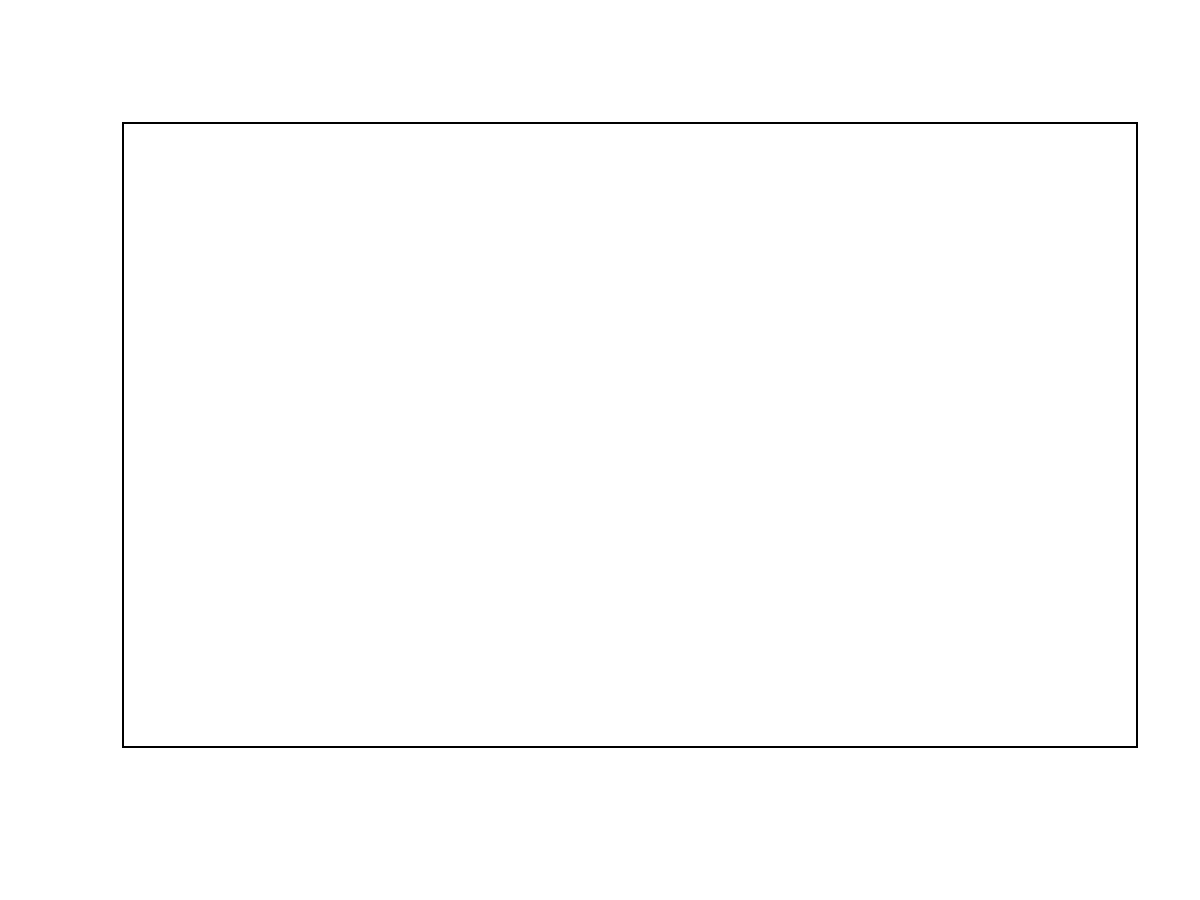
\includegraphics[width=4in, height=3in]{bamchop-pair-insert}
\caption{\textbf{Distribution of insertion size. }Insertion size is the distance between the mapping locations of the 5'-end of paired reads. It represents the size of DNA fragment to be sequenced.}
\end{SCfigure}
\end{center}

\pagebreak
\section{Base frequency}
This section summarizes the frequency of nucleic acid bases within sequencing reads in order to identify sequencing bias. 

\subsection{Base N frequency}
\begin{SCtable}[1][h!]
% latex table generated in R 2.15.2 by xtable 1.7-0 package
% Tue Apr 30 10:15:20 2013
\begin{tabular}{|r|r|r|r|}
  \hline
 & Total & N & Percentage \\ 
  \rowcolor[gray]{0.9} \hline
Base & 7,087,116 & 214 & 0.003 \\ 
  Read &   144,858 & 203 & 0.140 \\ 
   \hline
\end{tabular}\caption{\textbf{N base frequency.} The Ns in the reads are assigned by the sequencing machine to suggest that the base cannot be determined due to low quality or other reasons. This table shows the number and percentage of Ns and reads including any Ns. Ns are then excluded from the following analyses of base frequency. }
\end{SCtable}

\subsection{Expected vs. observed frequency}
\begin{SCtable}[1][h!]
% latex table generated in R 2.15.2 by xtable 1.7-0 package
% Tue Apr 30 10:15:20 2013
\begin{tabular}{|r|r|r|r|r|r|}
  \hline
 & A & C & G & T & GC \\ 
  \rowcolor[gray]{0.9} \hline
Expected(\%) & 29.51 &  20.47 &  20.48 & 29.55 &  40.94 \\ 
  Observed(\%) & 25.13 &  24.65 &  24.75 & 25.47 &  49.40 \\ 
   \rowcolor[gray]{0.9}Observed/Expected(\%) & 85.15 & 120.45 & 120.87 & 86.20 & 120.66 \\ 
   \hline
\end{tabular}\caption{\textbf{Expected vs. observed base frequency.} The expected base frequency is based on the whole reference genome and the observed frequency is the base frequency in sequencing reads. Their ratio reflects the sequencing bias of nucleic acid bases.}
\end{SCtable}

\subsection{GC content}
\begin{center}
\begin{SCfigure}[1][h!]
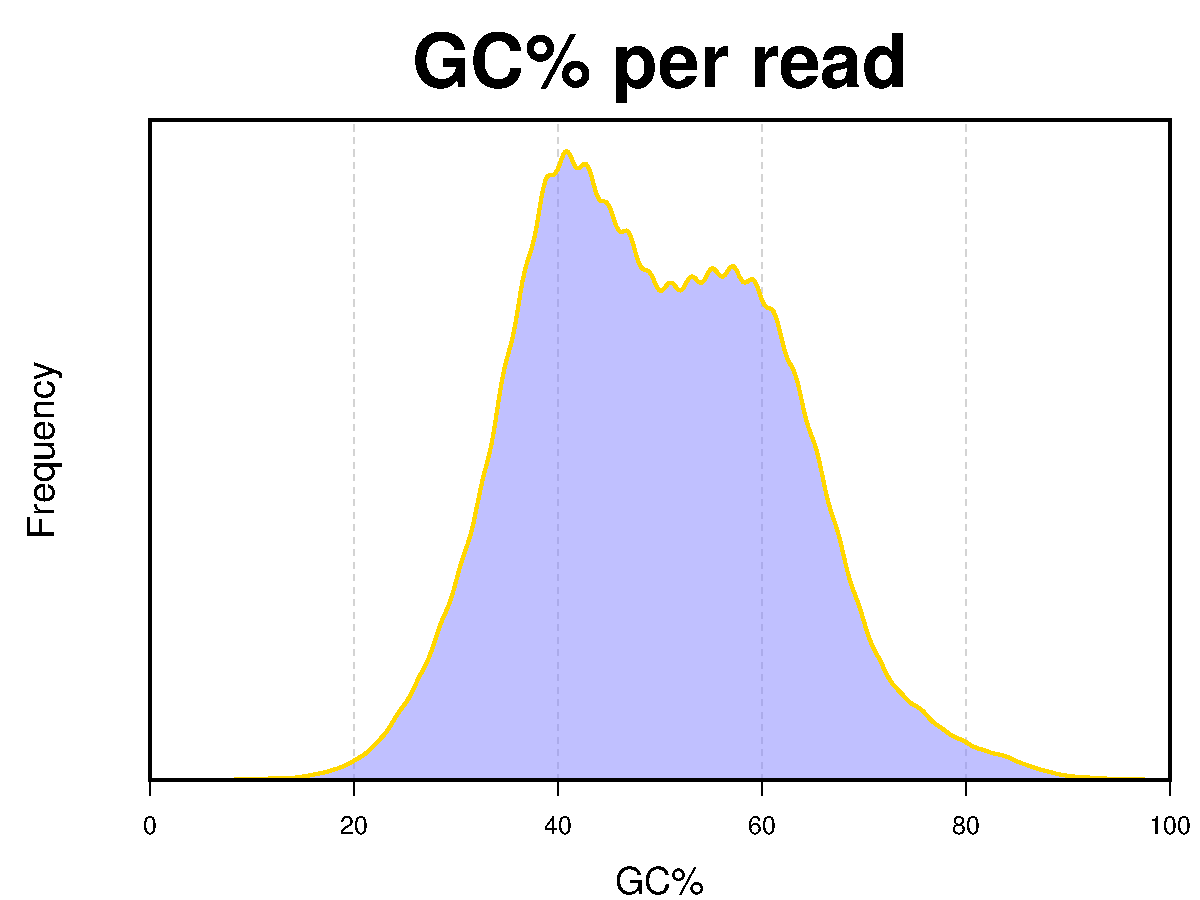
\includegraphics[width=3.2in, height=2.5in]{bamchop-base-gc}
\caption{\textbf{GC content.} Percentage of C/G bases within each read.}
\end{SCfigure}
\end{center}

\subsection{Position-specific base frequency}
Position-specific frequency of bases indicates whether there is a sequencing bias at both ends of the reads. The bias can be introduced via a variety of sources, such as DNA fragmentation and primer contamination. 
\subsubsection{Single base}
\begin{center}
\begin{figure}[h!]
\subfigure{
\includegraphics[width=3.33in, height=2in, page=2]{bamchop-base-fst-lst} }
\subfigure{
\includegraphics[width=3.33in, height=2in, page=4]{bamchop-base-fst-lst} }
\caption{\textbf{Single base frequency at both ends.}The base frequency of the first and last 10 bases (the rightmost is the last base) of reads. The frequency was normalized by the overall base frequency with sequencing reads, so this summary indicates the preference of sequencing to start with a given nucleic acid base.}
\end{figure}
\end{center}

\subsubsection{First two bases}

\begin{center}
\begin{SCfigure}[1][h!]
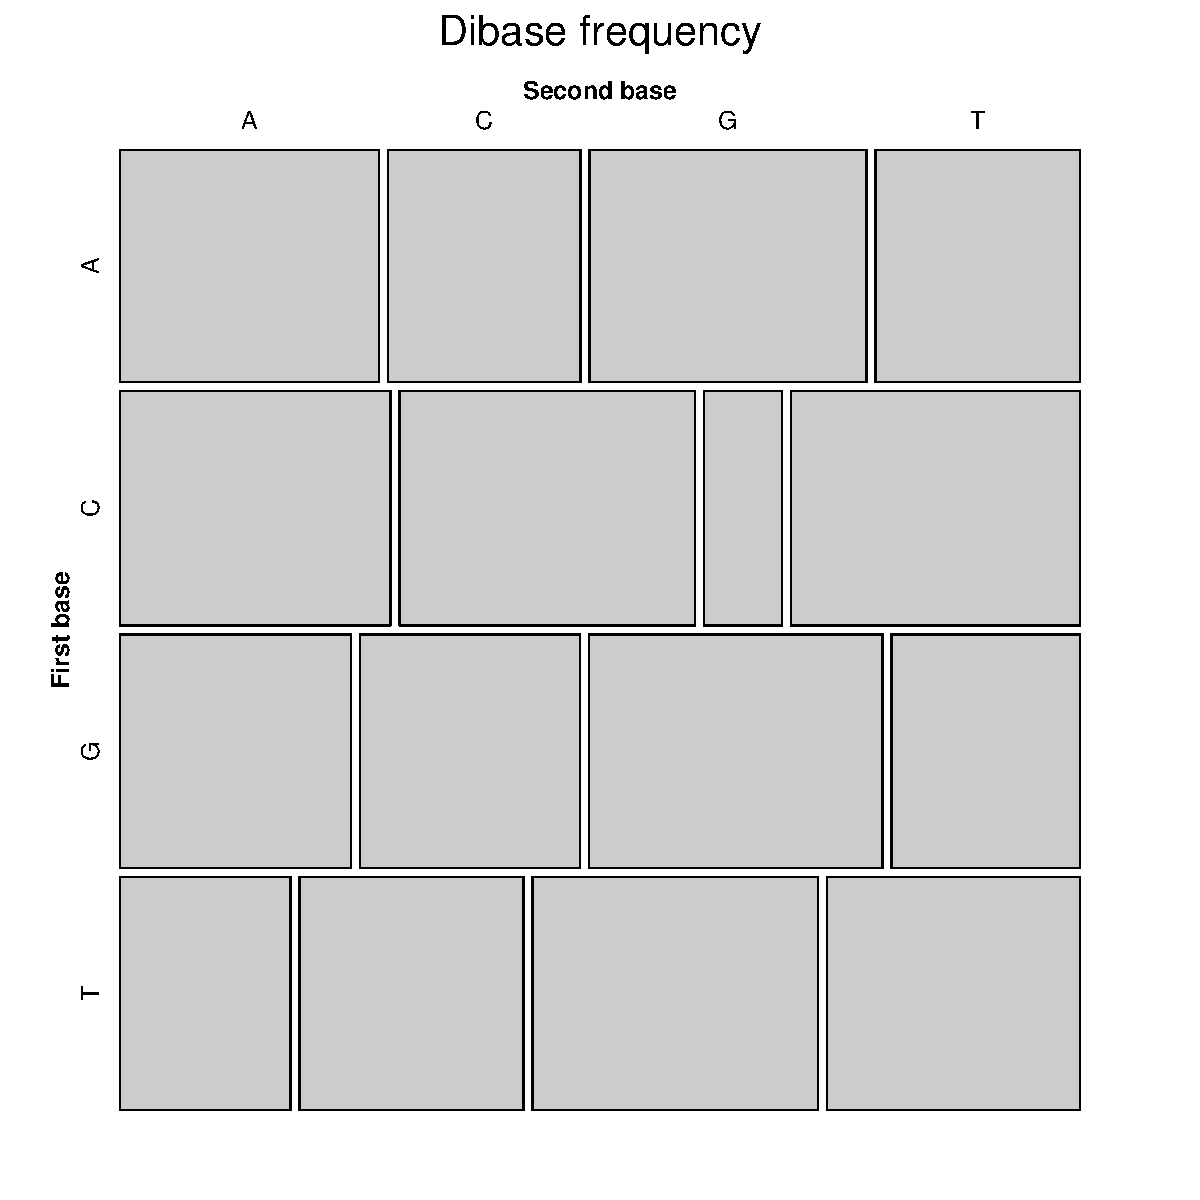
\includegraphics[width=2.5in, height=2.5in]{bamchop-base-two}
\caption{\textbf{First two base combination.}\small{This plot summarizes the frequency of the two-base combinations at the 5'-end of reads. The size of the blocks represent their relative frequency after adjusted by their expected frequency based on the position-specific frequency of the first two bases.}}
\end{SCfigure}
\end{center}

\subsubsection{5-mer frequency}
The frequency of 5-mer at both ends of reads.
\begin{center}
% latex table generated in R 2.15.2 by xtable 1.7-0 package
% Tue Apr 30 10:15:21 2013
{\scriptsize
\begin{longtable}{|r|r|r|r|}
\caption{Lowest frequency} \\ 
  \hline
5-mer & Expected\_count & Observed\_count & Observed/Expected \\ 
  \hline
CGTAC$|$ & 141.59 & 3 & 0.021 \\ 
   \rowcolor[gray]{0.9}TCGTA$|$ & 140.99 & 4 & 0.028 \\ 
  $|$TCGAC & 114.23 & 6 & 0.053 \\ 
   \rowcolor[gray]{0.9}$|$CGTAC & 146.54 & 6 & 0.041 \\ 
  CGATA$|$ & 142.12 & 6 & 0.042 \\ 
   \rowcolor[gray]{0.9}$|$TCCGA & 113.31 & 7 & 0.062 \\ 
  TACGA$|$ & 145.29 & 7 & 0.048 \\ 
   \rowcolor[gray]{0.9}GTACG$|$ & 140.47 & 8 & 0.057 \\ 
  GTCGT$|$ & 139.66 & 8 & 0.057 \\ 
   \rowcolor[gray]{0.9}CGTAT$|$ & 140.56 & 9 & 0.064 \\ 
   \hline
\hline
\end{longtable}
}% latex table generated in R 2.15.2 by xtable 1.7-0 package
% Tue Apr 30 10:15:21 2013
{\scriptsize
\begin{longtable}{|r|r|r|r|}
\caption{Highest frequency} \\ 
  \hline
5-mer & Expected\_count & Observed\_count & Observed/Expected \\ 
  \hline
$|$TTTTT & 165.92 & 732 & 4.41 \\ 
   \rowcolor[gray]{0.9}AAAAA$|$ & 151.23 & 685 & 4.53 \\ 
  TTTTT$|$ & 141.26 & 600 & 4.25 \\ 
   \rowcolor[gray]{0.9}$|$AAAAA & 162.51 & 556 & 3.42 \\ 
  $|$CCCAG & 115.92 & 517 & 4.46 \\ 
   \rowcolor[gray]{0.9}GAGGC$|$ & 142.95 & 467 & 3.27 \\ 
  $|$CTGGG & 150.42 & 462 & 3.07 \\ 
   \rowcolor[gray]{0.9}$|$CCAGG & 131.71 & 455 & 3.45 \\ 
  $|$GGTGG & 156.25 & 451 & 2.89 \\ 
   \rowcolor[gray]{0.9}GCCTC$|$ & 138.20 & 441 & 3.19 \\ 
   \hline
\hline
\end{longtable}
}% latex table generated in R 2.15.2 by xtable 1.7-0 package
% Tue Apr 30 10:15:21 2013
{\scriptsize
\begin{longtable}{|r|r|r|r|}
\caption{Highest relative enrichment} \\ 
  \hline
5-mer & Expected\_count & Observed\_count & Observed/Expected \\ 
  \hline
AAAAA$|$ & 151.23 & 685 & 4.53 \\ 
   \rowcolor[gray]{0.9}$|$CCCAG & 115.92 & 517 & 4.46 \\ 
  $|$TTTTT & 165.92 & 732 & 4.41 \\ 
   \rowcolor[gray]{0.9}TTTTT$|$ & 141.26 & 600 & 4.25 \\ 
  $|$CCAGG & 131.71 & 455 & 3.45 \\ 
   \rowcolor[gray]{0.9}$|$AAAAA & 162.51 & 556 & 3.42 \\ 
  GAGGC$|$ & 142.95 & 467 & 3.27 \\ 
   \rowcolor[gray]{0.9}CCTCC$|$ & 136.37 & 440 & 3.23 \\ 
  TCCTG$|$ & 136.62 & 438 & 3.21 \\ 
   \rowcolor[gray]{0.9}GCCTC$|$ & 138.20 & 441 & 3.19 \\ 
  $|$CTGGG & 150.42 & 462 & 3.07 \\ 
   \rowcolor[gray]{0.9}$|$CCTCC & 113.72 & 347 & 3.05 \\ 
  CCCAG$|$ & 135.89 & 409 & 3.01 \\ 
   \hline
\hline
\end{longtable}
}\end{center}
\newpage

\section{ChIP-seq}
This section of the report summarizes information related to a ChIP-seq experiment. 


\subsection{Strand-strand correlation}
Since sequencing usually starts from the 5-prime end of DNA fragments, reads mapped to the forward and reverse strands were skewed to the left and right respectively. While we expect a positive correlation between the two strands if reads were enriched around ChIP-ed regions, the forward strand needs to be shifted towards the right, or vice versa, to achieve the maximal strand correlation. The assoication between correlation coefficients and numbers of bases to shift indicates the distribution of DNA fragment sizes.


\begin{center}
\begin{figure}[H]
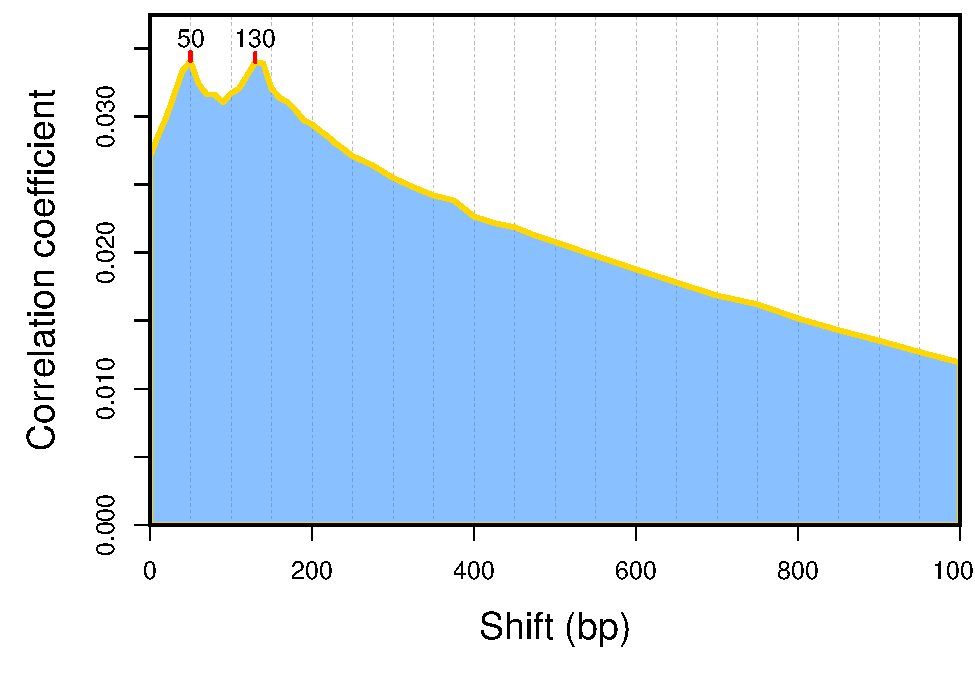
\includegraphics[width=6.5in, height=4.5in, page=1]{bamchop-chip-strand-corr}
\caption{\textbf{Strand-strand correlation vs. shifting.}The x-axis is the number of bases to shift the forward strand towards the right. Correlation was calculated between the 5-prime end of mapping locations after removing duplicated mappings.}
\end{figure}
\end{center}

\subsection{Peaks}
This section of the report is a quick summary of peaked regions without using specifically designed peak calling program. All reads were extended to  base pairs at the 3-prime end. A peak is defined here as a continuous region with at least 1X depth. 

\begin{SCtable}[1][h!]
% latex table generated in R 2.15.2 by xtable 1.7-0 package
% Tue Apr 30 10:15:21 2013
\begin{tabular}{|r|r|r|}
  \hline
Height & Count & Average\_width \\ 
  \rowcolor[gray]{0.9} \hline
$>$=10 & 17,098 & 1,831.46 \\ 
  $>$=25 & 10,648 & 2,155.48 \\ 
   \rowcolor[gray]{0.9}$>$=50 &  3,867 & 2,473.98 \\ 
  $>$=100 &    122 & 4,229.66 \\ 
   \rowcolor[gray]{0.9}$>$=200 &     50 & 5,604.08 \\ 
  $>$=500 &     32 & 5,505.34 \\ 
   \rowcolor[gray]{0.9}$>$=1,000 &     24 & 3,061.75 \\ 
  $>$=5,000 &      6 & 1,248.50 \\ 
   \rowcolor[gray]{0.9}$>$=10,000 &      3 &   649.67 \\ 
  =13,547 &      1 &   747.00 \\ 
   \hline
\end{tabular}\caption{\textbf{Peak summary.} Numbers of peaks with given depth and their average width.}
\end{SCtable}

\subsubsection{Peak height}
Peak height is the maximal sequencing depth within a peak.
\begin{center}
\begin{figure}[H]
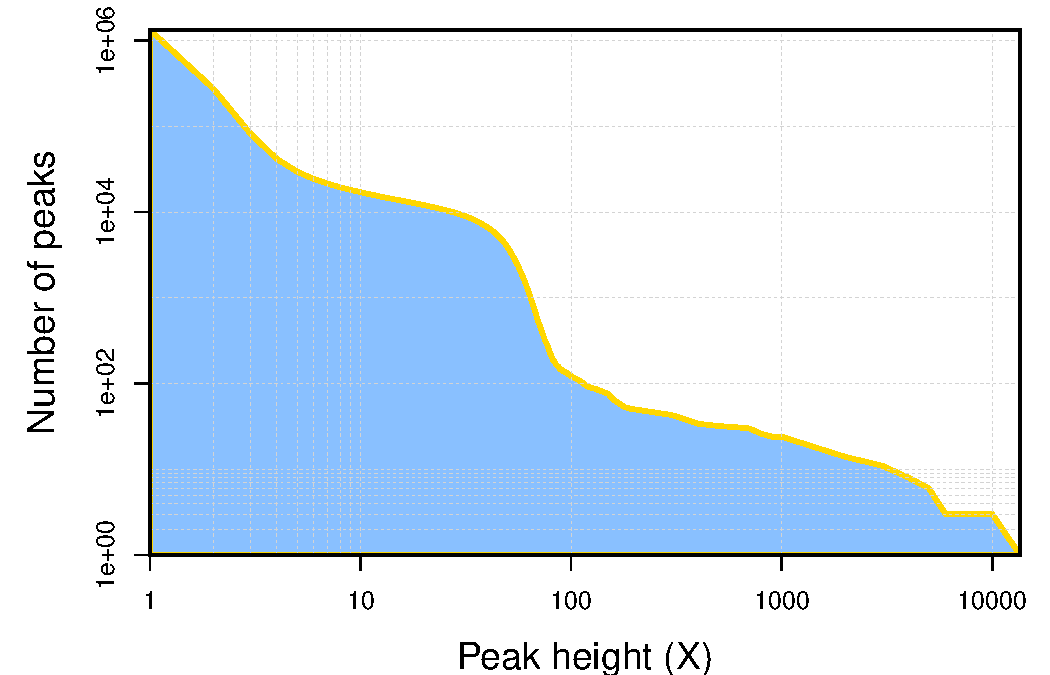
\includegraphics[width=7in, height=4.5in, page=1]{bamchop-chip-peak-height}
\caption{\textbf{Peak height distribution.}}
\end{figure}
\end{center}

\subsubsection{Peak width}
Peak width is the size of a continuous region with a minimum of 1X depth.
\vspace*{1\baselineskip}
\\{\textbf{Peak width summary:}}
\begin{Schunk}
\begin{Soutput}
   Min. 1st Qu.  Median    Mean 3rd Qu.    Max. 
  200.0   200.0   200.0   245.6   200.0 65710.0 
\end{Soutput}
\end{Schunk}


\begin{center}
\begin{figure}[H]
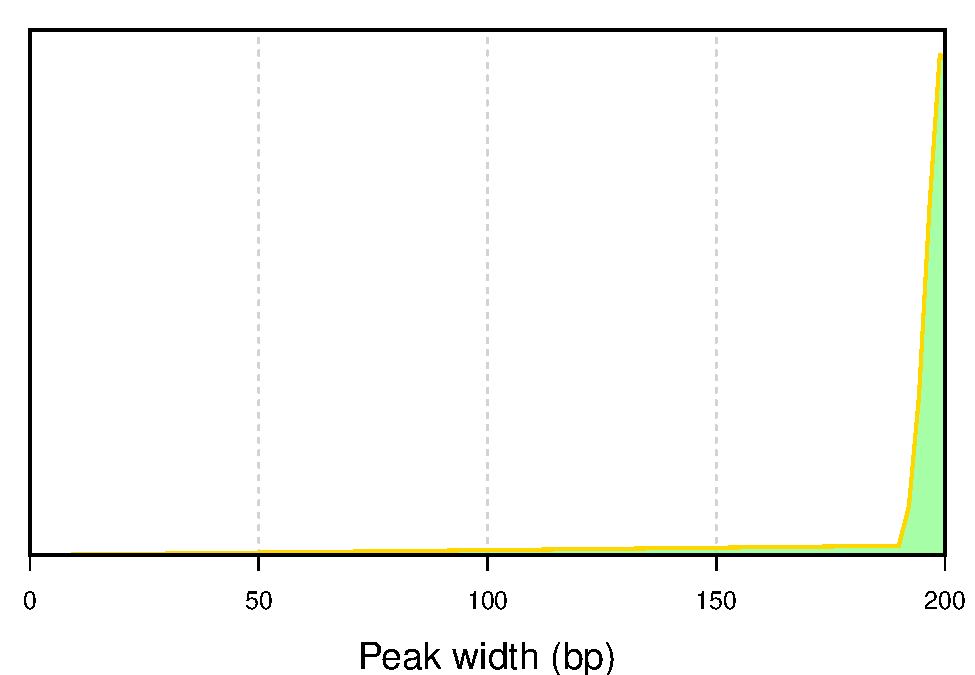
\includegraphics[width=6.5in, height=4.5in, page=1]{bamchop-chip-peak-width}
\caption{\textbf{Peak width distribution.}\small{}}
\end{figure}
\end{center}

\subsubsection{Peak frequency by genomic feature}
% latex table generated in R 2.15.2 by xtable 1.7-0 package
% Tue Apr 30 10:15:21 2013
{\tiny
\begin{longtable}{|r|r|r|r|r|r|r|}
\caption{Number of peaks mapped to genomic features.} \\ 
  \hline
Feature & Promoter & 5-UTR & Coding & Intron & 3-UTR & Exon \\ 
  \hline
Height$>$=10 & 12,040 & 11,267 & 8,747 & 13,090 & 906 & 12,605 \\ 
   \rowcolor[gray]{0.9}Height$>$=25 & 9,226 & 8,840 & 6,613 & 9,294 & 557 & 9,361 \\ 
  Height$>$=50 & 3,484 & 3,394 & 2,552 & 3,512 & 161 & 3,521 \\ 
   \rowcolor[gray]{0.9}Height$>$=100 & 17 & 5 & 5 & 38 &   1 & 21 \\ 
  Height$>$=200 & 3 & 0 & 0 & 14 &   0 & 3 \\ 
   \rowcolor[gray]{0.9}Height$>$=500 & 2 & 0 & 0 & 11 &   0 & 2 \\ 
  Height$>$=1000 & 2 & 0 & 0 & 11 &   0 & 2 \\ 
   \rowcolor[gray]{0.9}Height$>$=5000 & 1 & 0 & 0 & 3 &   0 & 1 \\ 
  Height$>$=10000 & 0 & 0 & 0 & 2 &   0 & 0 \\ 
   \rowcolor[gray]{0.9}Height$>$=13547 & 0 & 0 & 0 & 1 &   0 & 0 \\ 
   \hline
\hline
\end{longtable}
}
\begin{center}
\begin{figure}[H]
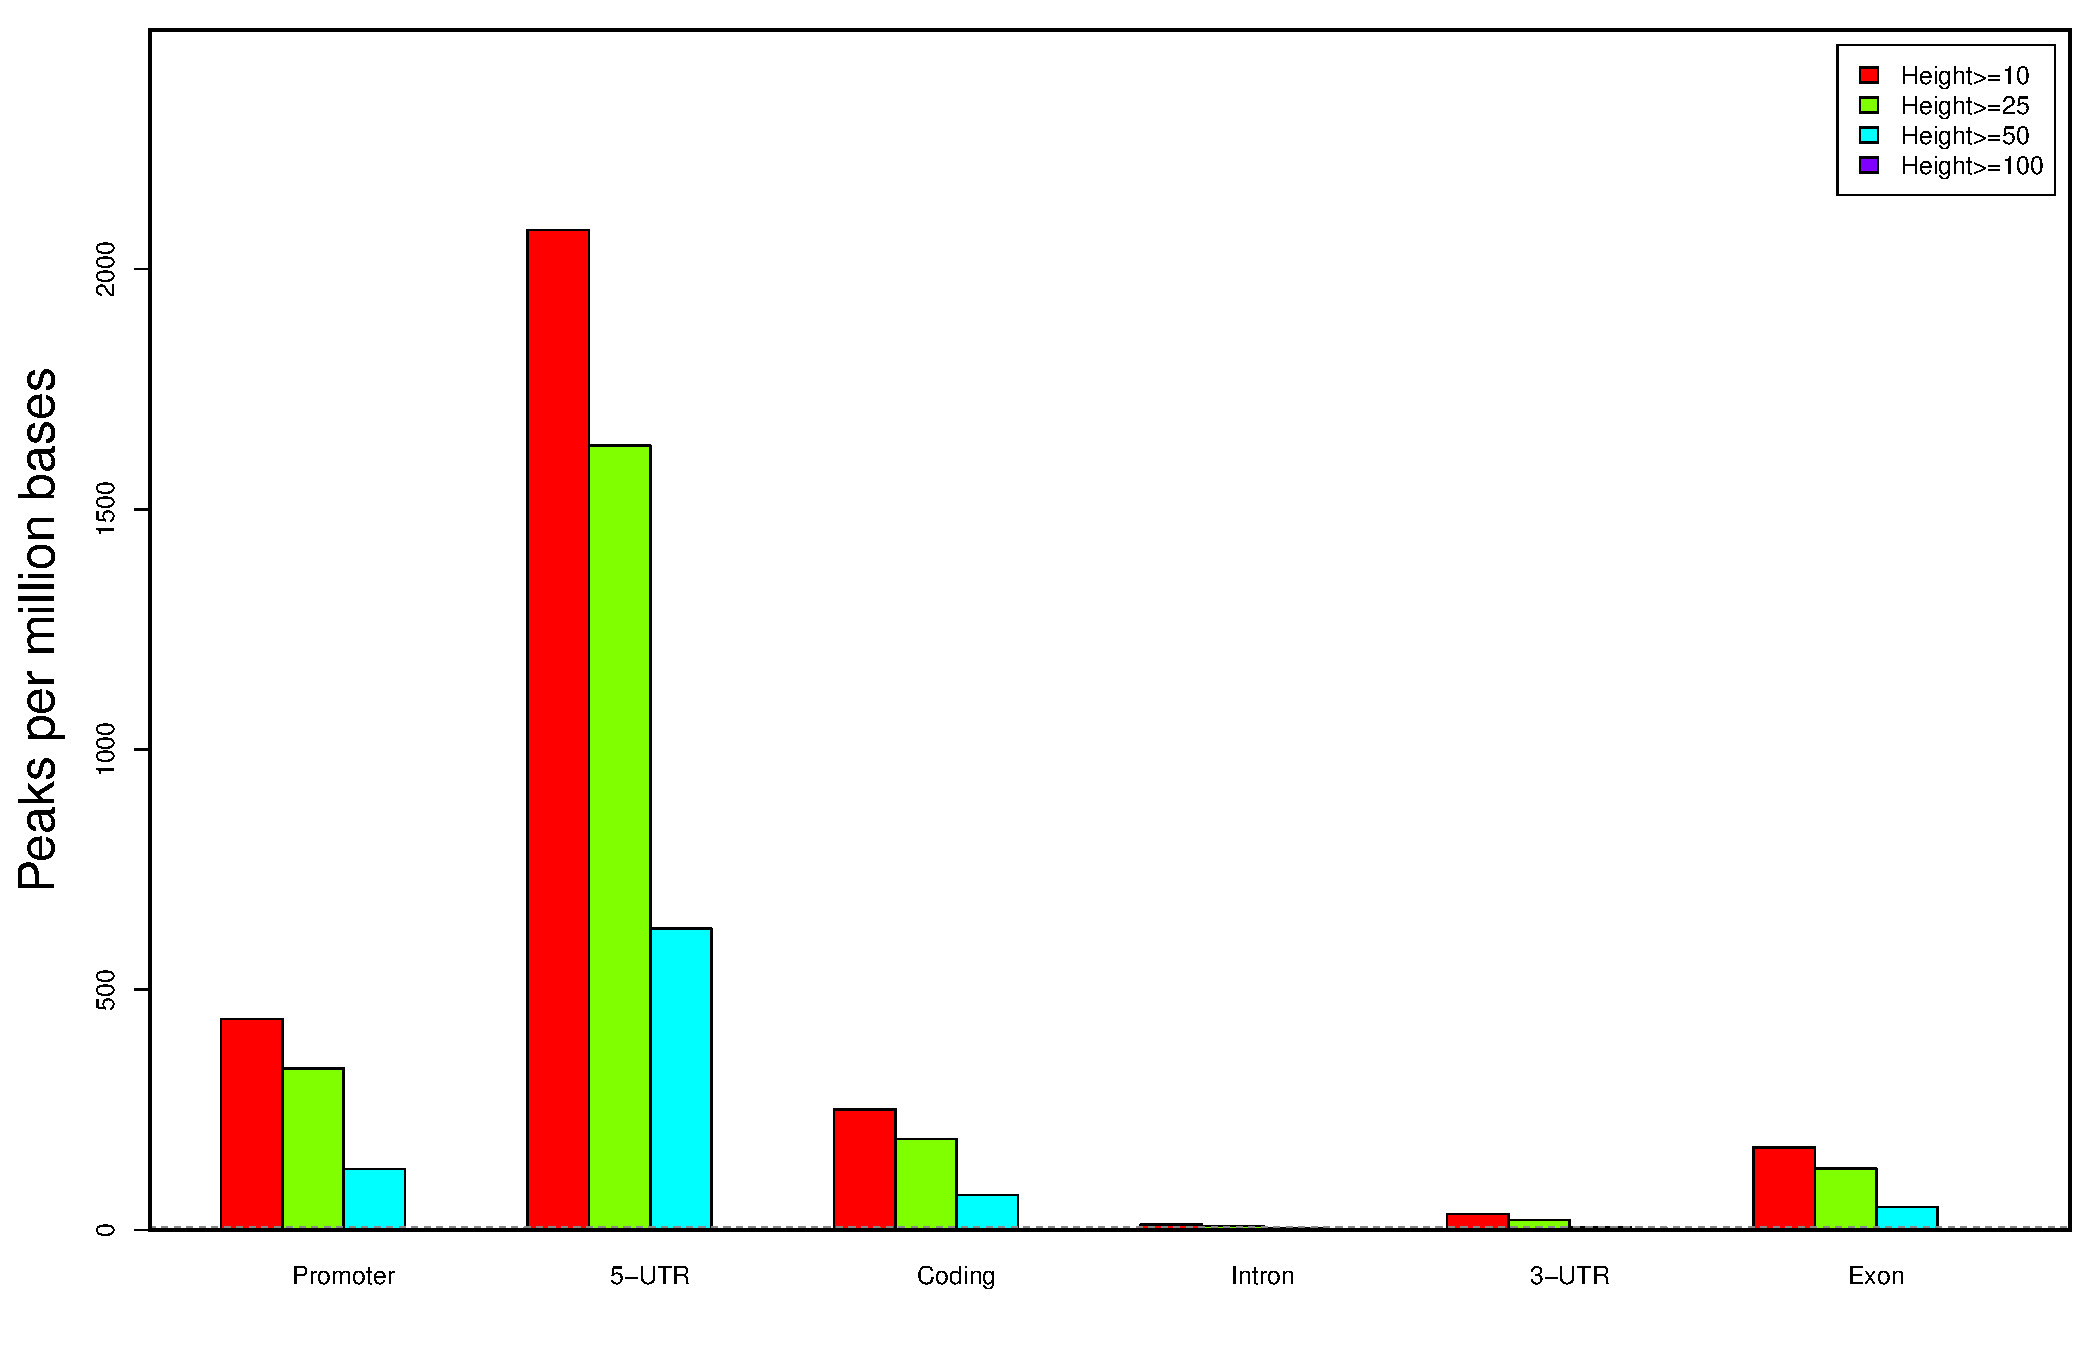
\includegraphics[width=7in, height=4.5in, page=1]{bamchop-chip-peak-by-feature}
\caption{\textbf{Peak frequency within genomic features.}The dashed line is the overall frequency of peaks with depth no less than 10 within the whole genome.}
\end{figure}
\end{center}

\subsubsection{Top peaks}
% latex table generated in R 2.15.2 by xtable 1.7-0 package
% Tue Apr 30 10:15:21 2013
{\scriptsize
\begin{longtable}{|r|r|r|r|r|}
\caption{Top 20 peaks with the highest height.} \\ 
  \hline
Chromosome & Start & End & Width & Height \\ 
  \hline
chr8 &  70,602,127 &  70,602,873 &   747 & 13,547 \\ 
   \rowcolor[gray]{0.9}chr4 &  70,296,441 &  70,296,928 &   488 & 10,331 \\ 
  chr1 &  91,852,605 &  91,853,318 &   714 & 10,030 \\ 
   \rowcolor[gray]{0.9}chr2 & 133,011,729 & 133,013,357 & 1,629 &  5,833 \\ 
  chr21 &   9,825,282 &   9,827,865 & 2,584 &  5,823 \\ 
   \rowcolor[gray]{0.9}chr19 &  24,183,922 &  24,185,250 & 1,329 &  5,476 \\ 
  chrX & 108,297,199 & 108,298,005 &   807 &  4,360 \\ 
   \rowcolor[gray]{0.9}chr12 &  20,704,189 &  20,704,657 &   469 &  4,276 \\ 
  chr19 &  36,066,337 &  36,066,971 &   635 &  3,424 \\ 
   \rowcolor[gray]{0.9}chr5 & 174,541,592 & 174,542,319 &   728 &  3,147 \\ 
  chr11 &  77,597,339 &  77,597,917 &   579 &  3,018 \\ 
   \rowcolor[gray]{0.9}chr16 &  33,960,491 &  33,966,645 & 6,155 &  2,616 \\ 
  chr1 & 121,478,264 & 121,485,604 & 7,341 &  2,384 \\ 
   \rowcolor[gray]{0.9}chr13 &  31,418,015 &  31,418,651 &   637 &  2,182 \\ 
  chr14 &  90,341,220 &  90,341,668 &   449 &  1,690 \\ 
   \rowcolor[gray]{0.9}chr1 & 145,277,112 & 145,277,800 &   689 &  1,634 \\ 
  chr1 & 120,543,550 & 120,544,263 &   714 &  1,517 \\ 
   \rowcolor[gray]{0.9}chr2 & 133,035,419 & 133,037,126 & 1,708 &  1,302 \\ 
  chr1 & 237,766,173 & 237,766,755 &   583 &  1,276 \\ 
   \rowcolor[gray]{0.9}chr2 &       9,836 &      10,356 &   521 &  1,264 \\ 
   \hline
\hline
\end{longtable}
}

\subsection{TSS}
This section of the report summarizes sequencing depth around transcription start sites (TSS).
\subsubsection{Strand-specific depth around TSS}
\begin{center}
\begin{figure}[H]
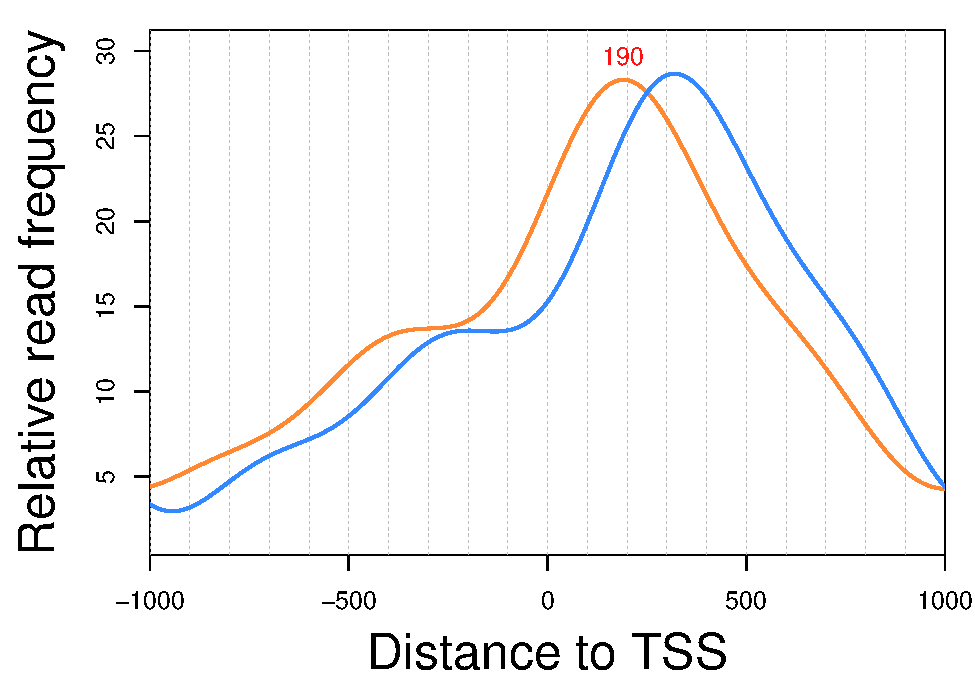
\includegraphics[width=6.5in, height=4.5in, page=1]{bamchop-chip-tss-loc}
\caption{\textbf{Read frequency around TSS.}This plot shows the frequency of reads whose 5-prime end was mapped around TSS of RefSeq genes. The read counts were normalized by the global average after duplicated mapping was not removed.}
\end{figure}
\end{center}

\subsubsection{Read counts around individual TSSs}
Read counts around TSS of individual genes.
\vspace*{1\baselineskip}
\\{\textbf{Read count summary:}}
\begin{Schunk}
\begin{Soutput}
   Min. 1st Qu.  Median    Mean 3rd Qu.    Max. 
   0.00    3.00   52.00   71.97  128.00  920.00 
\end{Soutput}
\end{Schunk}

\begin{center}
\begin{figure}[H]
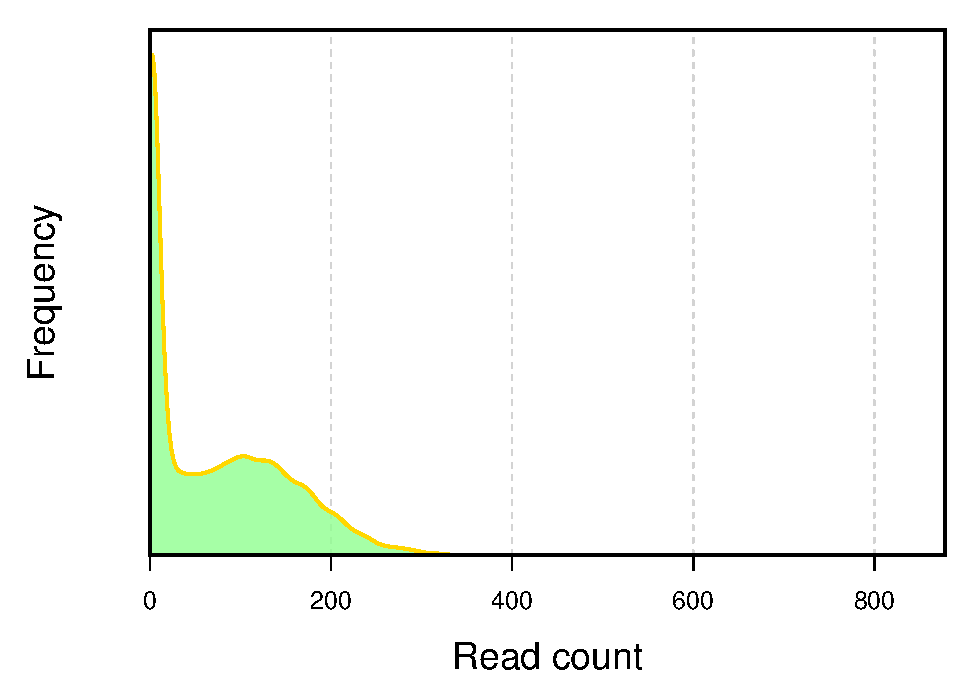
\includegraphics[width=6.5in, height=4.5in, page=1]{bamchop-chip-tss-gene}
\caption{\textbf{Read count distribution of genes.}This plot shows the distribution of read counts within the [-1kb, 1kb] region of RefSeq TSSs. Duplicated mapping was excluded.}
\end{figure}
\end{center}

% latex table generated in R 2.15.2 by xtable 1.7-0 package
% Tue Apr 30 10:15:21 2013
{\scriptsize
\begin{longtable}{|r|r|r|r|}
\caption{Top 20 genes with the highest read counts around TSS} \\ 
  \hline
RefSeq\_ID & Sense & Antisense & Total \\ 
  \hline
NR\_033770 & 460 & 460 & 920 \\ 
   \rowcolor[gray]{0.9}NR\_037458 & 433 & 453 & 886 \\ 
  NR\_037421 & 311 & 315 & 626 \\ 
   \rowcolor[gray]{0.9}NM\_203458 & 251 & 264 & 515 \\ 
  NR\_003264 & 256 & 225 & 481 \\ 
   \rowcolor[gray]{0.9}NM\_001200001 & 232 & 232 & 464 \\ 
  NM\_024408 & 232 & 232 & 464 \\ 
   \rowcolor[gray]{0.9}NR\_024077 & 201 & 190 & 391 \\ 
  NM\_001002811 & 203 & 182 & 385 \\ 
   \rowcolor[gray]{0.9}NR\_003265 & 192 & 191 & 383 \\ 
  NR\_029683 & 177 & 204 & 381 \\ 
   \rowcolor[gray]{0.9}NR\_040095 & 194 & 182 & 376 \\ 
  NM\_017940 & 167 & 191 & 358 \\ 
   \rowcolor[gray]{0.9}NM\_101395 & 187 & 166 & 353 \\ 
  NR\_003266 & 165 & 187 & 352 \\ 
   \rowcolor[gray]{0.9}NM\_014863 & 166 & 184 & 350 \\ 
  NM\_015892 & 166 & 184 & 350 \\ 
   \rowcolor[gray]{0.9}NM\_001024228 & 182 & 168 & 350 \\ 
  NM\_001024227 & 182 & 168 & 350 \\ 
   \rowcolor[gray]{0.9}NM\_001159673 & 164 & 164 & 328 \\ 
   \hline
\hline
\end{longtable}
}\newpage

\section{Alerts}
% latex table generated in R 2.15.2 by xtable 1.7-0 package
% Tue Apr 30 10:15:21 2013
 --- GC contents of reads are more than 110\% (120.7\%) of expected percentage. \\ 
  --- There are 13 5-mers overrepresented at either end of reads. \\ \end{document}
